\PassOptionsToPackage{enable-debug,check-declarations}{expl3}
\RequirePackage{pdfmanagement-testphase}
\DeclareDocumentMetadata {  }
\ExplSyntaxOn
\pdfmanagement_add:nnn{Catalog}{Lang}{(enUS)}
\ExplSyntaxOff

% xmp metadata for pdf
% Originally used \usepackage[a-2a]{pdfx}
% \usepackage{hyperxmp} replaced it
% \RequirePackage{pdfmanagement-testphase} replaced it

\documentclass[11pt,
  english,
  letterpaper,
]{article}
\usepackage{sa4ss}
\usepackage{amsmath,amssymb,array}
\usepackage{booktabs}

% From tagged-template.latex
\usepackage{lmodern}
\usepackage{ifxetex,ifluatex}
\ifnum 0\ifxetex 1\fi\ifluatex 1\fi=0 % if pdftex
  \usepackage[T1]{fontenc}
  \usepackage[utf8]{inputenc}
  \usepackage{textcomp} % provide euro and other symbols
\else % if luatex or xetex
  \usepackage{unicode-math}
  \defaultfontfeatures{Scale=MatchLowercase}
  \defaultfontfeatures[\rmfamily]{Ligatures=TeX,Scale=1}
\fi

% Use upquote if available, for straight quotes in verbatim environments
\IfFileExists{upquote.sty}{\usepackage{upquote}}{}
\IfFileExists{microtype.sty}{% use microtype if available
  \usepackage[]{microtype}
  \UseMicrotypeSet[protrusion]{basicmath} % disable protrusion for tt fonts
}{}
\makeatletter
\@ifundefined{KOMAClassName}{% if non-KOMA class
  \IfFileExists{parskip.sty}{%
    \usepackage{parskip}
  }{% else
    \setlength{\parindent}{0pt}
    \setlength{\parskip}{6pt plus 2pt minus 1pt}}
}{% if KOMA class
  \KOMAoptions{parskip=half}}
\makeatother
\usepackage{xcolor}
\IfFileExists{xurl.sty}{\usepackage{xurl}}{} % add URL line breaks if available
\hypersetup{
  pdftitle={DRAFT Rebuilding analysis for quillback rockfish (Sebastes maliger) in U.S. waters off the coast of California based on the 2021 stock assessment, incorporating November 2021 Council meeting requests},
  pdflang={en},
  hidelinks,
  pdfcreator={LaTeX via pandoc}}
\urlstyle{same} % disable monospaced font for URLs
\usepackage{longtable}
% Correct order of tables after \paragraph or \subparagraph
\usepackage{etoolbox}
\makeatletter
\patchcmd\longtable{\par}{\if@noskipsec\mbox{}\fi\par}{}{}
\makeatother
% Allow footnotes in longtable head/foot
\IfFileExists{footnotehyper.sty}{\usepackage{footnotehyper}}{\usepackage{footnote}}
\makesavenoteenv{longtable}
\usepackage{graphicx}
\makeatletter
\def\maxwidth{\ifdim\Gin@nat@width>\linewidth\linewidth\else\Gin@nat@width\fi}
\def\maxheight{\ifdim\Gin@nat@height>\textheight\textheight\else\Gin@nat@height\fi}
\makeatother
% Scale images if necessary, so that they will not overflow the page
% margins by default, and it is still possible to overwrite the defaults
% using explicit options in \includegraphics[width, height, ...]{}
\setkeys{Gin}{width=\maxwidth,height=\maxheight,keepaspectratio}
% Set default figure placement to htbp
\makeatletter
\def\fps@figure{htbp}
\makeatother
\setlength{\emergencystretch}{3em} % prevent overfull lines
\providecommand{\tightlist}{%
  \setlength{\itemsep}{0pt}\setlength{\parskip}{0pt}}
\setcounter{secnumdepth}{5}
\ifxetex
  % Load polyglossia as late as possible: uses bidi with RTL langages (e.g. Hebrew, Arabic)
  \usepackage{polyglossia}
  \setmainlanguage[]{english}
\else
  \usepackage[shorthands=off,main=english]{babel}
\fi

%Define cslreferences environment, required by pandoc 2.8
%https://github.com/rstudio/rmarkdown/issues/1649


\providecommand{\tightlist}{%
  \setlength{\itemsep}{0pt}\setlength{\parskip}{0pt}}


\date{}
\newcommand{\trTitle}{DRAFT Rebuilding analysis for quillback rockfish (\emph{Sebastes maliger}) in U.S. waters off the coast of California based on the 2021 stock assessment, incorporating November 2021 Council meeting requests}
\newcommand{\trYear}{2021}
\newcommand{\trMonth}{December}
\newcommand{\trAuthsLong}{true}
\newcommand{\trAuthsBack}{Langseth, B.J., C.R. Wetzel}
\newcommand{\trCitation}{
\begin{hangparas}{1em}{1}
\trAuthsBack{}. \trYear{}. \trTitle{}. \glsentrylong{pfmc}, Portland, Oregon. \pageref{LastPage}{}\,p.
\end{hangparas}}

\AtBeginDocument{\tagstructbegin{tag=Document}}
\AtEndDocument{\tagstructend}
\pretocmd{\maketitle}{\tagstructbegin{tag=H1}\tagmcbegin{tag=H1}}{}{}
\apptocmd{\maketitle}{\tagmcend\tagstructend}{}{}

\begin{document}

%%%%% Frontmatter %%%%%

% Footnote symbols in front matter
\renewcommand*{\thefootnote}{\fnsymbol{footnote}}

\small
\thispagestyle{empty}
\pagenumbering{roman}
\noindent
\begin{center}
\title{DRAFT Rebuilding analysis for quillback rockfish (\emph{Sebastes maliger}) in U.S. waters off the coast of California based on the 2021 stock assessment, incorporating November 2021 Council meeting requests}
% \textnormal{\MakeTextUppercase{\trTitle{}}}
\vspace{1.5cm}
{\Large\textbf\newline{DRAFT Rebuilding analysis for quillback rockfish (\emph{Sebastes maliger}) in U.S. waters off the coast of California based on the 2021 stock assessment, incorporating November 2021 Council meeting requests}}
\vfill
by\\
Brian J. Langseth\textsuperscript{1}\\
Chantel R. Wetzel\textsuperscript{1}\vfill
\textsuperscript{1}Northwest Fisheries Science Center, U.S. Department of Commerce, National Oceanic and Atmospheric Administration, National Marine Fisheries Service, 2725 Montlake Boulevard East, Seattle, Washington 98112\vfill
\trMonth{} \trYear{}
\end{center}
\clearpage

% Fourth page: Colophon
\thispagestyle{empty}
\vspace*{\fill}
\begin{center}
\copyright{} \glsentrylong{pfmc}, \trYear{}\\
\end{center}
\par
\bigskip
\noindent
Correct citation for this publication:
\bigskip
\par
\trCitation{}
\clearpage

% Add TOC to pdf bookmarks (clickable pdf)
\pdfbookmark[1]{\contentsname}{toc}

% Table of contents page, lists of figures and tables
\tableofcontents\clearpage
\label{TRlastRoman}
\clearpage

% Table of contents
\newpage
\thispagestyle{empty} % to remove page number

% Settings for the main document
\pagenumbering{arabic}  % Regular page numbers
\pagestyle{plain}  % No page number on first page of main document, use 'empty'
\renewcommand*{\thefootnote}{\arabic{footnote}}  % Back to numeric footnotes
\setcounter{footnote}{0}  % And start at 1
\renewcommand{\headrulewidth}{0.5pt}
\renewcommand{\footrulewidth}{0.5pt}
%\pagestyle{fancy}\fancyhead[c]{Draft: Do not cite or circulate}

\newcommand{\lt}{\ensuremath <}
\newcommand{\gt}{\ensuremath >}

\pagebreak
\pagenumbering{roman}
\setcounter{page}{1}

\renewcommand{\thetable}{\roman{table}}
\renewcommand{\thefigure}{\roman{figure}}

\setlength\parskip{0.5em plus 0.1em minus 0.2em}

\tagstructbegin{tag=H1}\tagmcbegin{tag=H1}

\hypertarget{disclaimer}{%
\section*{Disclaimer}\label{disclaimer}}
\addcontentsline{toc}{section}{Disclaimer}

\leavevmode\tagmcend\tagstructend

\tagstructbegin{tag=P}\tagmcbegin{tag=P}

\emph{These materials do not constitute a formal publication and are for information only. They are in a pre-review, pre-decisional state and should not be formally cited (or reproduced). They are to be considered provisional and do not represent any determination or policy of NOAA or the Department of Commerce.}

\leavevmode\tagmcend\tagstructend\par

\pagebreak

\tagstructbegin{tag=H1}\tagmcbegin{tag=H1}

\hypertarget{summary}{%
\section*{Summary}\label{summary}}
\addcontentsline{toc}{section}{Summary}

\leavevmode\tagmcend\tagstructend

\tagstructbegin{tag=P}\tagmcbegin{tag=P}

This rebuilding analysis is for the sub-stock of quillback rockfish (\emph{Sebastes maliger}) in waters off California. The analysis is based on the 2021 stock assessment {\tagstructbegin{tag=Reference}\tagmcbegin{tag=Reference}(Langseth et al. 2021)\leavevmode\tagmcend\tagstructend}. The 2021 assessment model estimated the quillback rockfish population to be at 14\% of the unexploited equilibrium spawning output at the start of 2021. This rebuilding analysis compares the results of applying a suite of potential management actions to the stock for 2023 and beyond.

\leavevmode\tagmcend\tagstructend\par

\tagstructbegin{tag=P}\tagmcbegin{tag=P}

This rebuilding analysis is an update of the one presented at the Pacific Fishery Management Council's (Council) November meeting, and incorporates the requests made by the Council during the November meeting. First, the assumed catch in 2022 was updated from 13.5 mt to 11.9 mt. Second, two SPR policies were added, at SPR = 0.55 and SPR = 0.65, as were two policies that delayed the application of constant SPR (at SPR = 0.6 and SPR = 0.7) until 2025. Third, the comparison between the base rebuilding analysis and the sensitivity rebuilding analyses with alternative assumptions about selectivity which was included in the November analysis was omitted for this report.

\leavevmode\tagmcend\tagstructend\par

\tagstructbegin{tag=P}\tagmcbegin{tag=P}

The results of the analysis show that the value for {\tagstructbegin{tag=Formula}\tagmcbegin{tag=Formula}\(\text{T}_\text{MIN}\)\leavevmode\tagmcend\tagstructend}, the median year for rebuilding to the target level in the absence of fishing since the year of declaration (2023), is 2040. The estimated generation time for quillback rockfish was estimated to be 26 years. In conjunction with {\tagstructbegin{tag=Formula}\tagmcbegin{tag=Formula}\(\text{T}_\text{MIN}\)\leavevmode\tagmcend\tagstructend} and the mean generation time, {\tagstructbegin{tag=Formula}\tagmcbegin{tag=Formula}\(\text{T}_\text{MAX}\)\leavevmode\tagmcend\tagstructend} was estimated to be 2066. An SPR = 0.577 harvest rate leads to a 50\% probability of recovery by {\tagstructbegin{tag=Formula}\tagmcbegin{tag=Formula}\(\text{T}_\text{MID}\)\leavevmode\tagmcend\tagstructend} where {\tagstructbegin{tag=Formula}\tagmcbegin{tag=Formula}\(\text{T}_\text{MID}\)\leavevmode\tagmcend\tagstructend} was 2053, an intermediate year between {\tagstructbegin{tag=Formula}\tagmcbegin{tag=Formula}\(\text{T}_\text{MIN}\)\leavevmode\tagmcend\tagstructend} and {\tagstructbegin{tag=Formula}\tagmcbegin{tag=Formula}\(\text{T}_\text{MAX}\)\leavevmode\tagmcend\tagstructend}.

\leavevmode\tagmcend\tagstructend\par

\pagebreak
\setlength{\parskip}{5mm plus1mm minus1mm}
\pagenumbering{arabic}
\setcounter{page}{1}
\renewcommand{\thefigure}{\arabic{figure}}
\renewcommand{\thetable}{\arabic{table}}
\setcounter{table}{0}
\setcounter{figure}{0}

\setlength\parskip{0.2em plus 0.1em minus 0.2em}

\tagstructbegin{tag=H1}\tagmcbegin{tag=H1}

\hypertarget{introduction}{%
\section{Introduction}\label{introduction}}

\leavevmode\tagmcend\tagstructend

\tagstructbegin{tag=P}\tagmcbegin{tag=P}

The 2021 assessment of quillback rockfish (\emph{Sebastes maliger}) in California waters documented that the population of quillback rockfish was below the Minimum Stock Size Threshold (MSST), which is 25\% of unfished spawning output for rockfish stocks, in 2021 {\tagstructbegin{tag=Reference}\tagmcbegin{tag=Reference}(Langseth et al. 2021)\leavevmode\tagmcend\tagstructend}. The population declined below MSST starting in 1992, reached it lowest values in the mid-1990s, increased to near the MSST in the 2000s and early 2010s, and declined in recent years. The stock is expected to be declared overfished for 2023 in 2021. Given the assumed productivity of the stock combined with the longevity of quillback rockfish a range of alternative rebuilding approaches were examined, and are described in this report, with rebuilding ranging from 2040 - 2064 based on various SPR harvest rates from 0.5 to 1 (no harvest).

\leavevmode\tagmcend\tagstructend\par

\tagstructbegin{tag=H1}\tagmcbegin{tag=H1}

\hypertarget{overview-of-the-2021-stock-assessment}{%
\section{Overview of the 2021 stock assessment}\label{overview-of-the-2021-stock-assessment}}

\leavevmode\tagmcend\tagstructend

\tagstructbegin{tag=P}\tagmcbegin{tag=P}

The 2021 assessment of quillback rockfish assessed the stock as three separate sub-stocks along the U.S. west coast: Washington, Oregon, and California. These were the first assessments of quillback rockfish conducted within Stock Synthesis {\tagstructbegin{tag=Reference}\tagmcbegin{tag=Reference}(Methot and Wetzel 2013)\leavevmode\tagmcend\tagstructend} that used catch and length composition data to inform model estimates around stock size and status. The previous assessment of quillback rockfish conducted in 2010 was a coastwide assessment modeled using Depletion-Based Stock Reduction Analysis (DB-SRA) to provide estimates of coastwide OFLs using catch data and biological information {\tagstructbegin{tag=Reference}\tagmcbegin{tag=Reference}(Dick and MacCall 2010)\leavevmode\tagmcend\tagstructend}. DB-SRA is a catch-only method and does not assess overfished status; the 2010 assessment assumed that current depletion was distributed around the management target of 40\%. The 2010 assessment found there was a 52\% chance that quillback rockfish was experiencing overfishing, as recent coastwide catch of quillback rockfish slightly exceeded the median coastwide OFL estimate at the time. Recent catches of quillback rockfish for the current assessment also exceed the ACL contributions for the species in all modeled areas.

\leavevmode\tagmcend\tagstructend\par

\tagstructbegin{tag=P}\tagmcbegin{tag=P}

Estimates of depletion in 2021 for the sub-stocks off Washington and Oregon were above the MSST threshold, but the estimate of depletion for the sub-stock off California was 14\%. See Langseth et al.~{\tagstructbegin{tag=Reference}\tagmcbegin{tag=Reference}(2021)\leavevmode\tagmcend\tagstructend} for additional results from the California quillback rockfish base model.

\leavevmode\tagmcend\tagstructend\par

\tagstructbegin{tag=P}\tagmcbegin{tag=P}

California quillback rockfish was assessed using a single-sex model with coastwide life history parameters combined across sexes. Life history parameters were estimated externally and then fixed within the model. Natural mortality and steepness were both fixed, at the median and mean of the priors, respectively. Annual recruitment deviations were estimated within the base model. The model for quillback rockfish in California waters included two fishing fleets, a commercial and a recreational fleet. The majority of the removals and length composition data arose from the recreational fleet. Recreational removals peaked in the late 1970s and early 1980s, with two years of large catches in 1984 and 1993. Removals declined sharply in 1994, but increased to levels similar to the late 1970s and early 1980s during the mid 2000s and again in recent years. Commercial removals peaked in the mid to late 1990s, with one year of exceptionally large catches in 1991. Removals declined through the mid 2010s, but increased in recent years. Selectivity for the commercial and recreational fleets was specified to be asymptotic. The assessment model decision table explored uncertainty around stock size and status using lower ({\tagstructbegin{tag=Formula}\tagmcbegin{tag=Formula}\(M\)\leavevmode\tagmcend\tagstructend} = 0.0464 yr{\tagstructbegin{tag=Formula}\tagmcbegin{tag=Formula}\(^{-1}\)\leavevmode\tagmcend\tagstructend}) and higher ({\tagstructbegin{tag=Formula}\tagmcbegin{tag=Formula}\(M\)\leavevmode\tagmcend\tagstructend} = 0.0744 yr{\tagstructbegin{tag=Formula}\tagmcbegin{tag=Formula}\(^{-1}\)\leavevmode\tagmcend\tagstructend}) natural mortality ({\tagstructbegin{tag=Formula}\tagmcbegin{tag=Formula}\(M\)\leavevmode\tagmcend\tagstructend}) values relative to the base model.

\leavevmode\tagmcend\tagstructend\par

\tagstructbegin{tag=P}\tagmcbegin{tag=P}

Sensitivities to modeling choices, catch history, and parameter values were explored and showed general support for the base model estimates of stock status and depletion. Sensitivities to the von Bertalanffy growth coefficient ({\tagstructbegin{tag=Formula}\tagmcbegin{tag=Formula}\(k\)\leavevmode\tagmcend\tagstructend}, whether estimated on its own or along with {\tagstructbegin{tag=Formula}\tagmcbegin{tag=Formula}\(L_\infty\)\leavevmode\tagmcend\tagstructend}) and natural mortality showed that model estimates of depletion were sensitive to these parameter choices.

\leavevmode\tagmcend\tagstructend\par

\tagstructbegin{tag=H1}\tagmcbegin{tag=H1}

\hypertarget{management-performance-under-rebuilding}{%
\section{Management performance under rebuilding}\label{management-performance-under-rebuilding}}

\leavevmode\tagmcend\tagstructend

\tagstructbegin{tag=P}\tagmcbegin{tag=P}

This is the first rebuilding plan for quillback rockfish in waters off the coast of California.

\leavevmode\tagmcend\tagstructend\par

\tagstructbegin{tag=H1}\tagmcbegin{tag=H1}

\hypertarget{rebuilding-calculations}{%
\section{Rebuilding calculations}\label{rebuilding-calculations}}

\leavevmode\tagmcend\tagstructend

\tagstructbegin{tag=P}\tagmcbegin{tag=P}

This rebuilding analysis was conducted in December, 2021 using software developed by A. Punt (version 3.12h, September 2021). The input file for the analysis is provided in {\tagstructbegin{tag=Link}\tagmcbegin{tag=Link}\protect\hyperlink{append_a}{Appendix A}\leavevmode\tagmcend\tagstructend}. The steps followed were:

\leavevmode\tagmcend\tagstructend\par

\begin{enumerate}
    \item Define how equilibrium spawning output ($\text{SB}_0$) will be calculated. 
    \item Define how future recruitment will be generated.
    \item Define the biological information on which future projections will be based.
    \item Define the fishery selectivity and allocation to be applied during rebuilding. 
    \item Decide how to include uncertainty in input parameters from the stock assessment in the rebuilding analysis. 
    \item Identification and analysis of alternative harvest strategies for rebuilding. 
\end{enumerate}

\tagstructbegin{tag=H2}\tagmcbegin{tag=H2}

\hypertarget{definition-of-equilibrium-spawning-output}{%
\subsection{Definition of Equilibrium Spawning Output}\label{definition-of-equilibrium-spawning-output}}

\leavevmode\tagmcend\tagstructend

\tagstructbegin{tag=P}\tagmcbegin{tag=P}

The equilibrium spawning output ({\tagstructbegin{tag=Formula}\tagmcbegin{tag=Formula}\(\text{SB}_0\)\leavevmode\tagmcend\tagstructend}) used in this rebuilding analysis is calculated via the stock-recruitment, growth, maturity, and fecundity relationships from the 2021 assessment in order to be consistent with assessment model results. Equilibrium spawning output was estimated to be 55.08 millions of eggs in the assessment model, which dictates a rebuilding relative spawning output target ({\tagstructbegin{tag=Formula}\tagmcbegin{tag=Formula}\(\text{SB}_{40\%}\)\leavevmode\tagmcend\tagstructend}) of 22.035 millions of eggs (Table \ref{tab:ref-points}). Estimates of spawning output presented in this report are female spawning output only.

\leavevmode\tagmcend\tagstructend\par

\tagstructbegin{tag=H2}\tagmcbegin{tag=H2}

\hypertarget{generation-of-future-recruitment}{%
\subsection{Generation of future recruitment}\label{generation-of-future-recruitment}}

\leavevmode\tagmcend\tagstructend

\tagstructbegin{tag=P}\tagmcbegin{tag=P}

The estimated parameters of the stock recruitment relationship including the unexploited equilibrium recruitment (natural log of {\tagstructbegin{tag=Formula}\tagmcbegin{tag=Formula}\(R_0\)\leavevmode\tagmcend\tagstructend} = 3.168), steepness ({\tagstructbegin{tag=Formula}\tagmcbegin{tag=Formula}\(h\)\leavevmode\tagmcend\tagstructend} = 0.72), and degree of recruitment variability ({\tagstructbegin{tag=Formula}\tagmcbegin{tag=Formula}\(\sigma_R = 0.60\)\leavevmode\tagmcend\tagstructend}) from the 2021 assessment were used to generate future recruitments in the rebuilding analysis.

\leavevmode\tagmcend\tagstructend\par

\tagstructbegin{tag=H2}\tagmcbegin{tag=H2}

\hypertarget{population-biology}{%
\subsection{Population biology}\label{population-biology}}

\leavevmode\tagmcend\tagstructend

\tagstructbegin{tag=P}\tagmcbegin{tag=P}

The biological parameters used for the rebuilding analysis were based on the values from the 2021 assessment. Biological parameters in the assessment were aggregated across sex and constant across time. The rebuilding analysis was based on a single sex model.

\leavevmode\tagmcend\tagstructend\par

\tagstructbegin{tag=H2}\tagmcbegin{tag=H2}

\hypertarget{fishery-selectivity-and-removal-allocations}{%
\subsection{Fishery selectivity, and removal allocations}\label{fishery-selectivity-and-removal-allocations}}

\leavevmode\tagmcend\tagstructend

\tagstructbegin{tag=P}\tagmcbegin{tag=P}

The selectivity used in the rebuilding analysis was obtained from the 2021 assessment. Selectivity in the assessment model was constant across time for each fishing fleet. The relative allocation of catch among fleets in the rebuilding analysis was informed using the relative fishing mortality from the assessment averaged over recent years (2017-2019). This choice provides some consistency between recent model results and forecasts from the rebuilding analysis, accounting for the unique dynamics in 2020 caused by the COVID-19 pandemic.

\leavevmode\tagmcend\tagstructend\par

\tagstructbegin{tag=H2}\tagmcbegin{tag=H2}

\hypertarget{inclusion-of-uncertainty}{%
\subsection{Inclusion of uncertainty}\label{inclusion-of-uncertainty}}

\leavevmode\tagmcend\tagstructend

\tagstructbegin{tag=P}\tagmcbegin{tag=P}

Model and parameter uncertainty is included in the rebuilding analysis via 1,000 random simulations of stochastic future recruitment strengths and integration over alternative low ({\tagstructbegin{tag=Formula}\tagmcbegin{tag=Formula}\(M\)\leavevmode\tagmcend\tagstructend} = 0.0464 yr{\tagstructbegin{tag=Formula}\tagmcbegin{tag=Formula}\(^{-1}\)\leavevmode\tagmcend\tagstructend}) and high ({\tagstructbegin{tag=Formula}\tagmcbegin{tag=Formula}\(M\)\leavevmode\tagmcend\tagstructend} = 0.0744 yr{\tagstructbegin{tag=Formula}\tagmcbegin{tag=Formula}\(^{-1}\)\leavevmode\tagmcend\tagstructend}) states of nature for values of natural mortality ({\tagstructbegin{tag=Formula}\tagmcbegin{tag=Formula}\(M\)\leavevmode\tagmcend\tagstructend}). Other potential states of nature were explored for the assessment, including for low and high ln({\tagstructbegin{tag=Formula}\tagmcbegin{tag=Formula}\(R_0\)\leavevmode\tagmcend\tagstructend}) and high and low {\tagstructbegin{tag=Formula}\tagmcbegin{tag=Formula}\(L_{\infty}\)\leavevmode\tagmcend\tagstructend}, but alternative values of natural mortality encapsulated a slightly wider range of depletion estimates compared to the other states of natures. The base model was given 50\% of the weight (500 simulations) and each alternative natural mortality state of nature was given 25\% (250 simulations) of the weight.

\leavevmode\tagmcend\tagstructend\par

\tagstructbegin{tag=H2}\tagmcbegin{tag=H2}

\hypertarget{alternate-rebuilding-strategies-analyzed}{%
\subsection{Alternate rebuilding strategies analyzed}\label{alternate-rebuilding-strategies-analyzed}}

\leavevmode\tagmcend\tagstructend

\tagstructbegin{tag=P}\tagmcbegin{tag=P}

Assuming that a constant rate of harvest will be applied throughout a rebuilding period, the basis for rebuilding alternatives can be divided into two approaches: 1) strategies based on selection of a constant harvest rate (SPR rate), or 2) strategies based on selection of a {\tagstructbegin{tag=Formula}\tagmcbegin{tag=Formula}\(\text{T}_\text{TARGET}\)\leavevmode\tagmcend\tagstructend} (year for 50\% probability of recovery). This rebuilding analysis presents the following alternate strategies, which are a combination of those specified in the rebuilding Terms of Reference (TOR; PFMC {\tagstructbegin{tag=Reference}\tagmcbegin{tag=Reference}(2020)\leavevmode\tagmcend\tagstructend}) and additional strategies. The additional strategies are based on the selection of a SPR harvest rate, rebuilding by a selected target year, or by delaying a SPR harvest rate for a specified number of years.

\leavevmode\tagmcend\tagstructend\par

\begin{enumerate}
    \item Eliminate all harvest, F = 0, starting in the next management cycle, 2023, the same as setting a constant SPR harvest rate of 1.0.
    \item Apply the harvest rate that would generate the ACL contributions specified for the current year (i.e., the latest year specified in regulations). 
    \item Apply a range of SPR values: 
    \begin{enumerate}
     \item SPR = 0.50,
     \item SPR = 0.55
     \item SPR = 0.60,
     \item SPR = 0.65,
     \item SPR = 0.70,
     \item SPR = 0.80, and
     \item SPR = 0.90. 
    \end{enumerate}
    \item Apply a range of SPR values to start in 2025 to allow a ramp down in fishing pressure from 2023-2025:
    \begin{enumerate}
     \item SPR = 0.60, and
     \item SPR = 0.7.
    \end{enumerate}
    \item Apply SPR harvest rates that are estimated to lead to a 50$\%$ probability of recovery by alternative target years: 
    \begin{enumerate}
     \item by $\text{T}_\text{MAX}$ from the current cycle, and 
     \item by $\text{T}_\text{MID}$ from the current cycle, which is the year midway between $\text{T}_\text{MIN}$ and $\text{T}_\text{MAX}$.
    \end{enumerate}
    \item Apply the default harvest policy based on the 40:10 harvest control rule with time-varying sigma ($\sigma$ = 1.0 as the basis for the time-varying sigmas) and $P^*$ = 0.45.
    \item Apply the ABC harvest rate with time-varying sigma ($\sigma$ = 1.0 as the basis for the time-varying sigmas) and $P^*$ = 0.45.
\end{enumerate}

\tagstructbegin{tag=P}\tagmcbegin{tag=P}

The sum of ACL contributions for quillback rockfish from the southern management area and the percent allocation for California (28.7{\tagstructbegin{tag=Formula}\tagmcbegin{tag=Formula}\(\%\)\leavevmode\tagmcend\tagstructend}) in the northern management area as provided by the Groundfish Management Team (GMT) were larger than the catch resulting from applying an SPR of 0.5, implying an SPR rate of below 0.5 for this run, so results from this strategy are not provided in this report. Similarly, the SPR rate that led to a 50{\tagstructbegin{tag=Formula}\tagmcbegin{tag=Formula}\(\%\)\leavevmode\tagmcend\tagstructend} probability of recovery by {\tagstructbegin{tag=Formula}\tagmcbegin{tag=Formula}\(\text{T}_\text{MAX}\)\leavevmode\tagmcend\tagstructend} was less than 0.5 so results from the {\tagstructbegin{tag=Formula}\tagmcbegin{tag=Formula}\(\text{T}_\text{MAX}\)\leavevmode\tagmcend\tagstructend} strategy are not presented in this report.

\leavevmode\tagmcend\tagstructend\par

\tagstructbegin{tag=P}\tagmcbegin{tag=P}

No current rebuilding plan exists for quillback rockfish in California waters so the alternatives related to the results of a previous rebuilding plan as specified in the rebuilding TOR could not be done. These include:

\leavevmode\tagmcend\tagstructend\par

\begin{itemize}
 \item Apply the spawning potential ratio or relevant harvest control run in the current rebuilding plan. 
 \item Apply the harvest rate that is estimated to lead to a 50$\%$ probability of recovery by the current $\text{T}_\text{TARGET}$.
 \item Apply the harvest rate that is estimated to lead to a 50$\%$ probability of recovery by the $\text{T}_\text{MAX}$ from the previous cycle.
\end{itemize}

\tagstructbegin{tag=P}\tagmcbegin{tag=P}

All of the above rebuilding strategies were conducted assuming removals of 13.5 mt in 2021 and 11.9 mt in 2022 as recommended by the GMT.

\leavevmode\tagmcend\tagstructend\par

\tagstructbegin{tag=H3}\tagmcbegin{tag=H3}

\hypertarget{ramp-strategies}{%
\subsubsection{Ramp strategies}\label{ramp-strategies}}

\leavevmode\tagmcend\tagstructend

\tagstructbegin{tag=P}\tagmcbegin{tag=P}

The Council requested ``ramp-down'' strategies be explored that gradually reduced catches from 2022 values over a three year period. Two strategies were explored using constant SPR = 0.6 and SPR = 0.7 rates starting in 2025. For these ramp-down strategies, catch in 2023 was set equal to the catch in 2023 indicated under the ABC harvest rate strategy. Catches in 2024 were iteratively set to be approximately midway between the 2023 ABC-based catch value and the estimated catch in 2025 from the corresponding SPR strategy (SPR = 0.6 or SPR = 0.7) starting in 2024 with fixed 2023 catch, and therefore reflects a linear ramp in catch between 2023-2025. Catch in 2024 was further adjusted as necessary, to ensure a declining ramp, meaning that the change in catch between 2023-2024 was greater than or equal to the change in catch between 2024-2025.

\leavevmode\tagmcend\tagstructend\par

\tagstructbegin{tag=H1}\tagmcbegin{tag=H1}

\hypertarget{results}{%
\section{Results}\label{results}}

\leavevmode\tagmcend\tagstructend

\tagstructbegin{tag=H2}\tagmcbegin{tag=H2}

\hypertarget{rebuilding-reference-points}{%
\subsection{Rebuilding reference points}\label{rebuilding-reference-points}}

\leavevmode\tagmcend\tagstructend

\tagstructbegin{tag=P}\tagmcbegin{tag=P}

Reference points calculated based on this rebuilding analysis are given in Table \ref{tab:ref-points}. The minimum time required for rebuilding, {\tagstructbegin{tag=Formula}\tagmcbegin{tag=Formula}\(\text{T}_\text{MIN}\)\leavevmode\tagmcend\tagstructend}, with no fishing (F=0) starting in 2023 was estimated to be 17 years, corresponding to the stock being rebuilt by 2040, assuming the default removals for 2021 and 2022. The mean generation time was estimated to be 26 years. The maximum time allowed for rebuilding, {\tagstructbegin{tag=Formula}\tagmcbegin{tag=Formula}\(\text{T}_\text{MAX}\)\leavevmode\tagmcend\tagstructend}, is defined as the {\tagstructbegin{tag=Formula}\tagmcbegin{tag=Formula}\(\text{T}_\text{MIN}\)\leavevmode\tagmcend\tagstructend} plus the mean generation time for stocks that require more than 10 years to rebuild. Quillback rockfish was unable to rebuild within 10 years so the estimated {\tagstructbegin{tag=Formula}\tagmcbegin{tag=Formula}\(\text{T}_\text{MAX}\)\leavevmode\tagmcend\tagstructend} was 2066. {\tagstructbegin{tag=Formula}\tagmcbegin{tag=Formula}\(\text{T}_\text{TARGET}\)\leavevmode\tagmcend\tagstructend}, and {\tagstructbegin{tag=Formula}\tagmcbegin{tag=Formula}\(\text{SPR}_\text{TARGET}\)\leavevmode\tagmcend\tagstructend} are not specified since this is the first rebuilding plan for quillback rockfish and these values have not been set via the Council's process.

\leavevmode\tagmcend\tagstructend\par

\tagstructbegin{tag=P}\tagmcbegin{tag=P}

A rebuilding strategy is presented below and includes a rebuilding target year termed {\tagstructbegin{tag=Formula}\tagmcbegin{tag=Formula}\(\text{T}_\text{MID}\)\leavevmode\tagmcend\tagstructend}, which equals 2053 and is the mid-point between {\tagstructbegin{tag=Formula}\tagmcbegin{tag=Formula}\(\text{T}_\text{MIN}\)\leavevmode\tagmcend\tagstructend} and {\tagstructbegin{tag=Formula}\tagmcbegin{tag=Formula}\(\text{T}_\text{MAX}\)\leavevmode\tagmcend\tagstructend}. The Council may opt to select a {\tagstructbegin{tag=Formula}\tagmcbegin{tag=Formula}\(\text{T}_\text{TARGET}\)\leavevmode\tagmcend\tagstructend} earlier or later than this {\tagstructbegin{tag=Formula}\tagmcbegin{tag=Formula}\(\text{T}_\text{MID}\)\leavevmode\tagmcend\tagstructend} value based on fishery, economic, or other factors.

\leavevmode\tagmcend\tagstructend\par

\tagstructbegin{tag=H2}\tagmcbegin{tag=H2}

\hypertarget{alternative-harvest-policy-projections}{%
\subsection{Alternative harvest policy projections}\label{alternative-harvest-policy-projections}}

\leavevmode\tagmcend\tagstructend

\tagstructbegin{tag=P}\tagmcbegin{tag=P}

Summary results from the rebuilding alternatives are presented in Table \ref{tab:reb-options}. Results from the ramp-down strategies are presented in Table \ref{tab:reb-ramp-options}. Detailed results for all runs are presented in Tables \ref{tab:prob-mat}-\ref{tab:rel-ssb-mat} and Figures \ref{fig:prob-fig}-\ref{fig:ssb-fig}.

\leavevmode\tagmcend\tagstructend\par

\tagstructbegin{tag=P}\tagmcbegin{tag=P}

The target rebuilding year based on the various rebuilding strategies ranged from 2040 - 2064 (Tables \ref{tab:reb-options} and \ref{tab:reb-ramp-options}). The probability of rebuilding by year steadily increased across the alternative SPR values with full rebuilding (reaching a probability of greater than 50\%) by 2064 when the lowest SPR of 0.50 was applied (Table \ref{tab:prob-mat} and Figure \ref{fig:prob-fig}). The recommended removals in 2023, the first year of rebuilding, were low ranging between 0.12 - 2.11 mt across strategies excluding the no-harvest strategy (Table \ref{tab:acl-mat}), with the recommended removals slowly increasing by year during the rebuilding period (Figure \ref{fig:acl-fig}). The estimated Overfishing Limits (OFLs) for each rebuilding alternative are given in Table \ref{tab:ofl-mat}. The change in spawning output by year relative to the spawning output target, 40\% of unfished, under each of the alternatives are shown by year in Table \ref{tab:rel-ssb-mat} and Figure \ref{fig:rel-ssb-fig}. The harvest rate to obtain a 50\% probability of recovery by {\tagstructbegin{tag=Formula}\tagmcbegin{tag=Formula}\(\text{T}_\text{MAX}\)\leavevmode\tagmcend\tagstructend} corresponds to an SPR that is lower than 0.5, so is not provided in the tables.

\leavevmode\tagmcend\tagstructend\par

\tagstructbegin{tag=H1}\tagmcbegin{tag=H1}

\hypertarget{acknowledgements}{%
\section{Acknowledgements}\label{acknowledgements}}

\leavevmode\tagmcend\tagstructend

\tagstructbegin{tag=P}\tagmcbegin{tag=P}

Andre Punt (University of Washington) updated the rebuilder program to apply time-varying {\tagstructbegin{tag=Formula}\tagmcbegin{tag=Formula}\(\sigma\)\leavevmode\tagmcend\tagstructend} for the Acceptable Biological Catch and 40-10 scenarios. Andre Punt and Owen Hamel (NOAA) provided assistance in understanding and applying the rebuilder program. Owen Hamel provided comments on early drafts of the analysis.

\leavevmode\tagmcend\tagstructend\par

\clearpage

\tagstructbegin{tag=H1}\tagmcbegin{tag=H1}

\hypertarget{references}{%
\section{References}\label{references}}

\leavevmode\tagmcend\tagstructend

\tagstructbegin{tag=BibEntry}\tagmcbegin{tag=BibEntry}

\hypertarget{refs}{}
\leavevmode\hypertarget{ref-DickandMacCall_dbsra_2010}{}%
Dick, E.J., and MacCall, A.D. 2010. Estimates of sustainable yield for 50 data-poor stocks in the pacfici coast groundfish fishery management plot. NOAA Tech. Memo, NOAA-TM-NMFS-SWFSC-460.

\leavevmode\hypertarget{ref-Langseth_status_2021}{}%
Langseth, B.J., Wetzel, C.R., Cope, J.M., and Budrick, J.E. 2021. Status of quillback rockfish (\emph{Sebastes maliger}) in U.S. Waters off the coast of california in 2021 using catch and length data. Pacific Fishery Management Council, 7700 Ambassador Place NE, Suite 200, Portland, OR 97220.

\leavevmode\hypertarget{ref-methot_stock_2013}{}%
Methot, R.D., and Wetzel, C.R. 2013. Stock synthesis: A biological and statistical framework for fish stock assessment and fishery management. Fisheries Research 142: 86--99.

\leavevmode\hypertarget{ref-TOR_2020}{}%
Pacific Fishery Management Council (PFMC). 2020. Terms of reference for the groundfish and coastal pelagic species stock assessment review process for 2021-2022. Pacific Fishery Management Council, 7700 Ambassador Place NE, Suite 200, Portland, OR 97220.

\leavevmode\tagmcend\tagstructend

\clearpage

\tagstructbegin{tag=H1}\tagmcbegin{tag=H1}

\hypertarget{tables}{%
\section{Tables}\label{tables}}

\leavevmode\tagmcend\tagstructend

\tagstructbegin{tag=H2}\tagmcbegin{tag=H2}

\hypertarget{rebuilding-reference-points-and-policy-projections}{%
\subsection{Rebuilding reference points and policy projections}\label{rebuilding-reference-points-and-policy-projections}}

\leavevmode\tagmcend\tagstructend

\begingroup\fontsize{10}{12}\selectfont
\begingroup\fontsize{10}{12}\selectfont

\tagstructbegin{tag=Table}\tagmcbegin{tag=Table}
\begin{longtable}[t]{l>{\raggedright\arraybackslash}p{2cm}}
\caption{\label{tab:ref-points}Summary of the rebuilding reference points.}\\
\toprule
Quantity & 2021 Assessment Values\\
\midrule
\endfirsthead
\caption[]{\label{tab:ref-points}Summary of the rebuilding reference points. \textit{(continued)}}\\
\toprule
Quantity & 2021 Assessment Values\\
\midrule
\endhead

\endfoot
\bottomrule
\endlastfoot
SB0 (millions of eggs) & 55.08\\
SB40 (millions of eggs) & 22.035\\
SB2021 (millions of eggs) & 7.745\\
Year rebuilding begins & 2023\\
Current year & 2021\\
T\textsubscript{MIN} & 2040\\
Mean generation time (years) & 26\\
T\textsubscript{MAX} & 2066\\
T\textsubscript{F=0} & 2040\\
T\textsubscript{TARGET} & TBD\\
SPR\textsubscript{TARGET} & TBD\\
Current SPR (2021) & 0.1165\\*
\end{longtable}
\leavevmode\tagmcend\tagstructend\par
\endgroup{}
\endgroup{}

\begingroup\fontsize{10}{12}\selectfont

\begin{landscape}\begingroup\fontsize{10}{12}\selectfont

\tagstructbegin{tag=Table}\tagmcbegin{tag=Table}
\begin{longtable}[t]{l>{\raggedright\arraybackslash}p{0.92cm}>{\raggedright\arraybackslash}p{0.92cm}>{\raggedright\arraybackslash}p{0.92cm}>{\raggedright\arraybackslash}p{0.92cm}>{\raggedright\arraybackslash}p{0.92cm}>{\raggedright\arraybackslash}p{0.92cm}>{\raggedright\arraybackslash}p{0.92cm}>{\raggedright\arraybackslash}p{0.92cm}>{\raggedright\arraybackslash}p{0.92cm}>{\raggedright\arraybackslash}p{0.92cm}>{\raggedright\arraybackslash}p{0.92cm}}
\caption{\label{tab:reb-options}Results of rebuilding alternatives based on alternative SPR targets for 50 percent probability of recovery based on the assumed removals for 2021-22. SPR for the ABC and 40-10 strategies is provided as a dash (-) because these strategies do not have a constant SPR value}\\
\toprule
 & SPR= .500       & SPR= .550       & SPR= .600       & SPR= .650       & SPR= .700       & SPR= .800       & SPR= .900       & Yr= T\textsubscript{MID} & F=0             & 40-10 rule      & ABC Rule       \\
\midrule
\endfirsthead
\caption[]{\label{tab:reb-options}Results of rebuilding alternatives based on alternative SPR targets for 50 percent probability of recovery based on the assumed removals for 2021-22. SPR for the ABC and 40-10 strategies is provided as a dash (-) because these strategies do not have a constant SPR value \textit{(continued)}}\\
\toprule
 & SPR= .500       & SPR= .550       & SPR= .600       & SPR= .650       & SPR= .700       & SPR= .800       & SPR= .900       & Yr= T\textsubscript{MID} & F=0             & 40-10 rule      & ABC Rule       \\
\midrule
\endhead

\endfoot
\bottomrule
\endlastfoot
2021 Assumed Removals (mt) & 13.5 & 13.5 & 13.5 & 13.5 & 13.5 & 13.5 & 13.5 & 13.5 & 13.5 & 13.5 & 13.5\\
2022 Assumed Removals (mt) & 11.9 & 11.9 & 11.9 & 11.9 & 11.9 & 11.9 & 11.9 & 11.9 & 11.9 & 11.9 & 11.9\\
2023 ACL (mt) & 2.11 & 1.76 & 1.46 & 1.2 & 0.97 & 0.58 & 0.26 & 1.59 & 0 & 0.12 & 1.84\\
2024 ACL (mt) & 2.3 & 1.93 & 1.61 & 1.33 & 1.08 & 0.65 & 0.29 & 1.76 & 0 & 0.41 & 2\\
SPR & 0.5 & 0.55 & 0.6 & 0.65 & 0.7 & 0.8 & 0.9 & 0.577 & 1 & - & -\\
T\textsubscript{TARGET} & 2064 & 2057 & 2051 & 2048 & 2046 & 2043 & 2041 & 2053 & 2040 & 2051 & 2055\\
T\textsubscript{MAX} & 2066 & 2066 & 2066 & 2066 & 2066 & 2066 & 2066 & 2066 & 2066 & 2066 & 2066\\
Probability of recovery by T\textsubscript{MAX} & 0.536 & 0.788 & 0.905 & 0.948 & 0.98 & 0.999 & 1 & 0.851 & 1 & 0.906 & 0.83\\*
\end{longtable}
\leavevmode\tagmcend\tagstructend\par
\endgroup{}
\end{landscape}
\endgroup{}
\clearpage

\begingroup\fontsize{10}{12}\selectfont

\begin{landscape}\begingroup\fontsize{10}{12}\selectfont

\tagstructbegin{tag=Table}\tagmcbegin{tag=Table}
\begin{longtable}[t]{l>{\raggedright\arraybackslash}p{2.2cm}>{\raggedright\arraybackslash}p{2.2cm}>{\raggedright\arraybackslash}p{2.2cm}>{\raggedright\arraybackslash}p{2.2cm}}
\caption{\label{tab:reb-ramp-options}Results of rebuilding alternatives for ramp-down strategies (ramp) based on applying alternative SPR targets starting in 2025 for 50 percent probability of recovery based on assumed removals for 2021-22 and fixed removals in 2023-24. Non-ramp strategies are copied from Table \ref{tab:reb-options} and included for comparison. Catches in 2023-2024 for non-ramp strategies were estimated based on the specified SPR value, and were not fixed}\\
\toprule
 & Ramp SPR = .600 & SPR = .600 & Ramp SPR = .700 & SPR = .700\\
\midrule
\endfirsthead
\caption[]{\label{tab:reb-ramp-options}Results of rebuilding alternatives for ramp-down strategies (ramp) based on applying alternative SPR targets starting in 2025 for 50 percent probability of recovery based on assumed removals for 2021-22 and fixed removals in 2023-24. Non-ramp strategies are copied from Table \ref{tab:reb-options} and included for comparison. Catches in 2023-2024 for non-ramp strategies were estimated based on the specified SPR value, and were not fixed \textit{(continued)}}\\
\toprule
 & Ramp SPR = .600 & SPR = .600 & Ramp SPR = .700 & SPR = .700\\
\midrule
\endhead

\endfoot
\bottomrule
\endlastfoot
2021 Assumed Removals (mt) & 13.5 & 13.5 & 13.5 & 13.5\\
2022 Assumed Removals (mt) & 11.9 & 11.9 & 11.9 & 11.9\\
2023 Fixed Removals (mt), (2023 ACL for non-ramp) & 1.84 & 1.46 & 1.84 & 0.97\\
2024 Fixed Removals (mt), (2024 ACL for non-ramp) & 1.8 & 1.61 & 1.5 & 1.08\\
2025 ACL (mt) & 1.76 & 1.78 & 1.17 & 1.2\\
SPR in 2025 & 0.6 & 0.6 & 0.7 & 0.7\\
T\textsubscript{TARGET} & 2051 & 2051 & 2046 & 2046\\
Probability of recovery by T\textsubscript{MAX} = 2066 & 0.896 & 0.905 & 0.979 & 0.98\\*
\end{longtable}
\leavevmode\tagmcend\tagstructend\par
\endgroup{}
\end{landscape}
\endgroup{}
\clearpage

\tagstructbegin{tag=H2}\tagmcbegin{tag=H2}

\hypertarget{rebuilding-time-series}{%
\subsection{Rebuilding time series}\label{rebuilding-time-series}}

\leavevmode\tagmcend\tagstructend

\begingroup\fontsize{10}{12}\selectfont
\begingroup\fontsize{10}{12}\selectfont

\tagstructbegin{tag=Table}\tagmcbegin{tag=Table}
\begin{longtable}[t]{l>{\raggedright\arraybackslash}p{0.79cm}>{\raggedright\arraybackslash}p{0.79cm}>{\raggedright\arraybackslash}p{0.79cm}>{\raggedright\arraybackslash}p{0.79cm}>{\raggedright\arraybackslash}p{0.79cm}>{\raggedright\arraybackslash}p{0.79cm}>{\raggedright\arraybackslash}p{0.79cm}>{\raggedright\arraybackslash}p{0.79cm}>{\raggedright\arraybackslash}p{0.79cm}>{\raggedright\arraybackslash}p{0.79cm}>{\raggedright\arraybackslash}p{0.79cm}>{\raggedright\arraybackslash}p{0.79cm}>{\raggedright\arraybackslash}p{0.79cm}}
\caption{\label{tab:prob-mat}Probability of recovery by year for rebuilding strategies, including ramp strategies. Probabilities represent the proportion of simulations that reach the target biomass by the specified year}\\
\toprule
Year & SPR= .500       & SPR= .550 & SPR= .600       & Ramp SPR= .600 & SPR= .650 & SPR= .700       & Ramp SPR= .700 & SPR= .800       & SPR= .900       & Yr= T\textsubscript{MID} & F=0             & 40-10 rule      & ABC Rule       \\
\midrule
\endfirsthead
\caption[]{\label{tab:prob-mat}Probability of recovery by year for rebuilding strategies, including ramp strategies. Probabilities represent the proportion of simulations that reach the target biomass by the specified year \textit{(continued)}}\\
\toprule
Year & SPR= .500       & SPR= .550 & SPR= .600       & Ramp SPR= .600 & SPR= .650 & SPR= .700       & Ramp SPR= .700 & SPR= .800       & SPR= .900       & Yr= T\textsubscript{MID} & F=0             & 40-10 rule      & ABC Rule       \\
\midrule
\endhead

\endfoot
\bottomrule
\endlastfoot
2021 & 0.000 & 0.000 & 0.000 & 0.000 & 0.000 & 0.000 & 0.000 & 0.000 & 0.000 & 0.000 & 0.000 & 0.000 & 0.000\\
2022 & 0.000 & 0.000 & 0.000 & 0.000 & 0.000 & 0.000 & 0.000 & 0.000 & 0.000 & 0.000 & 0.000 & 0.000 & 0.000\\
2023 & 0.000 & 0.000 & 0.000 & 0.000 & 0.000 & 0.000 & 0.000 & 0.000 & 0.000 & 0.000 & 0.000 & 0.000 & 0.000\\
2024 & 0.000 & 0.000 & 0.000 & 0.000 & 0.000 & 0.000 & 0.000 & 0.000 & 0.000 & 0.000 & 0.000 & 0.000 & 0.000\\
2025 & 0.000 & 0.000 & 0.000 & 0.000 & 0.000 & 0.000 & 0.000 & 0.000 & 0.000 & 0.000 & 0.000 & 0.000 & 0.000\\
2026 & 0.000 & 0.000 & 0.000 & 0.000 & 0.000 & 0.000 & 0.000 & 0.000 & 0.000 & 0.000 & 0.000 & 0.000 & 0.000\\
2027 & 0.000 & 0.000 & 0.000 & 0.000 & 0.000 & 0.000 & 0.000 & 0.000 & 0.000 & 0.000 & 0.000 & 0.000 & 0.000\\
2028 & 0.000 & 0.000 & 0.000 & 0.000 & 0.000 & 0.000 & 0.000 & 0.000 & 0.000 & 0.000 & 0.000 & 0.000 & 0.000\\
2029 & 0.000 & 0.000 & 0.000 & 0.000 & 0.000 & 0.001 & 0.001 & 0.001 & 0.001 & 0.000 & 0.005 & 0.000 & 0.000\\
2030 & 0.000 & 0.001 & 0.001 & 0.001 & 0.001 & 0.003 & 0.004 & 0.007 & 0.011 & 0.001 & 0.018 & 0.001 & 0.001\\
2031 & 0.001 & 0.002 & 0.003 & 0.004 & 0.004 & 0.010 & 0.010 & 0.018 & 0.042 & 0.003 & 0.080 & 0.003 & 0.002\\
2032 & 0.002 & 0.003 & 0.008 & 0.010 & 0.014 & 0.020 & 0.022 & 0.053 & 0.111 & 0.005 & 0.163 & 0.006 & 0.003\\
2033 & 0.004 & 0.009 & 0.016 & 0.022 & 0.031 & 0.048 & 0.050 & 0.104 & 0.175 & 0.012 & 0.220 & 0.013 & 0.009\\
2034 & 0.009 & 0.017 & 0.033 & 0.040 & 0.055 & 0.081 & 0.086 & 0.161 & 0.211 & 0.027 & 0.236 & 0.028 & 0.018\\
2035 & 0.014 & 0.033 & 0.050 & 0.052 & 0.073 & 0.115 & 0.121 & 0.191 & 0.235 & 0.042 & 0.256 & 0.048 & 0.034\\
2036 & 0.023 & 0.039 & 0.063 & 0.072 & 0.102 & 0.154 & 0.153 & 0.216 & 0.251 & 0.052 & 0.283 & 0.057 & 0.046\\
2037 & 0.028 & 0.052 & 0.085 & 0.087 & 0.131 & 0.174 & 0.175 & 0.238 & 0.287 & 0.065 & 0.325 & 0.074 & 0.055\\
2038 & 0.031 & 0.061 & 0.102 & 0.106 & 0.158 & 0.191 & 0.193 & 0.273 & 0.332 & 0.083 & 0.386 & 0.094 & 0.071\\
2039 & 0.034 & 0.072 & 0.123 & 0.130 & 0.177 & 0.234 & 0.234 & 0.318 & 0.387 & 0.102 & 0.455 & 0.114 & 0.085\\
2040 & 0.045 & 0.091 & 0.143 & 0.152 & 0.217 & 0.284 & 0.279 & 0.366 & 0.438 & 0.118 & 0.530 & 0.142 & 0.102\\
2041 & 0.055 & 0.104 & 0.181 & 0.185 & 0.257 & 0.321 & 0.311 & 0.414 & 0.504 & 0.146 & 0.602 & 0.177 & 0.117\\
2042 & 0.069 & 0.132 & 0.208 & 0.214 & 0.292 & 0.358 & 0.353 & 0.455 & 0.575 & 0.169 & 0.663 & 0.210 & 0.149\\
2043 & 0.081 & 0.149 & 0.244 & 0.246 & 0.331 & 0.402 & 0.390 & 0.518 & 0.631 & 0.201 & 0.708 & 0.248 & 0.166\\
2044 & 0.095 & 0.173 & 0.283 & 0.282 & 0.364 & 0.435 & 0.430 & 0.575 & 0.675 & 0.231 & 0.742 & 0.285 & 0.198\\
2045 & 0.109 & 0.197 & 0.319 & 0.321 & 0.406 & 0.470 & 0.464 & 0.621 & 0.722 & 0.263 & 0.764 & 0.321 & 0.229\\
2046 & 0.125 & 0.228 & 0.353 & 0.352 & 0.433 & 0.528 & 0.513 & 0.659 & 0.750 & 0.307 & 0.798 & 0.355 & 0.265\\
2047 & 0.141 & 0.260 & 0.378 & 0.377 & 0.474 & 0.559 & 0.553 & 0.700 & 0.780 & 0.336 & 0.837 & 0.389 & 0.304\\
2048 & 0.153 & 0.293 & 0.409 & 0.405 & 0.517 & 0.601 & 0.597 & 0.739 & 0.815 & 0.363 & 0.863 & 0.429 & 0.330\\
2049 & 0.170 & 0.324 & 0.442 & 0.442 & 0.555 & 0.633 & 0.627 & 0.776 & 0.849 & 0.388 & 0.898 & 0.455 & 0.354\\
2050 & 0.194 & 0.347 & 0.481 & 0.481 & 0.582 & 0.675 & 0.658 & 0.812 & 0.879 & 0.417 & 0.925 & 0.491 & 0.381\\
2051 & 0.216 & 0.371 & 0.507 & 0.504 & 0.614 & 0.717 & 0.710 & 0.840 & 0.910 & 0.447 & 0.940 & 0.524 & 0.415\\
2052 & 0.232 & 0.405 & 0.535 & 0.534 & 0.658 & 0.759 & 0.742 & 0.868 & 0.921 & 0.479 & 0.961 & 0.554 & 0.442\\
2053 & 0.250 & 0.432 & 0.565 & 0.556 & 0.700 & 0.790 & 0.775 & 0.889 & 0.940 & 0.500 & 0.975 & 0.589 & 0.471\\
2054 & 0.280 & 0.453 & 0.598 & 0.591 & 0.733 & 0.819 & 0.803 & 0.910 & 0.962 & 0.525 & 0.981 & 0.635 & 0.494\\
2055 & 0.298 & 0.477 & 0.640 & 0.627 & 0.768 & 0.845 & 0.829 & 0.925 & 0.976 & 0.555 & 0.989 & 0.665 & 0.517\\
2056 & 0.321 & 0.497 & 0.668 & 0.659 & 0.797 & 0.865 & 0.854 & 0.943 & 0.977 & 0.604 & 0.993 & 0.700 & 0.554\\
2057 & 0.339 & 0.533 & 0.694 & 0.688 & 0.825 & 0.887 & 0.873 & 0.958 & 0.987 & 0.637 & 0.997 & 0.722 & 0.588\\
2058 & 0.361 & 0.566 & 0.725 & 0.717 & 0.846 & 0.901 & 0.895 & 0.967 & 0.992 & 0.660 & 1.000 & 0.761 & 0.622\\
2059 & 0.386 & 0.597 & 0.754 & 0.740 & 0.865 & 0.926 & 0.912 & 0.971 & 0.996 & 0.689 & 1.000 & 0.781 & 0.650\\
2060 & 0.405 & 0.624 & 0.771 & 0.765 & 0.889 & 0.935 & 0.929 & 0.982 & 0.997 & 0.712 & 1.000 & 0.802 & 0.677\\
2061 & 0.429 & 0.649 & 0.805 & 0.793 & 0.898 & 0.949 & 0.939 & 0.988 & 0.998 & 0.740 & 1.000 & 0.824 & 0.707\\
2062 & 0.459 & 0.684 & 0.831 & 0.822 & 0.916 & 0.955 & 0.950 & 0.995 & 0.999 & 0.762 & 1.000 & 0.849 & 0.730\\
2063 & 0.479 & 0.703 & 0.855 & 0.847 & 0.921 & 0.963 & 0.959 & 0.997 & 0.999 & 0.791 & 1.000 & 0.868 & 0.756\\
2064 & 0.502 & 0.726 & 0.872 & 0.863 & 0.935 & 0.965 & 0.964 & 0.998 & 0.999 & 0.824 & 1.000 & 0.884 & 0.788\\
2065 & 0.511 & 0.754 & 0.888 & 0.878 & 0.942 & 0.973 & 0.968 & 0.998 & 0.999 & 0.840 & 1.000 & 0.899 & 0.815\\
2066 & 0.536 & 0.788 & 0.905 & 0.896 & 0.948 & 0.980 & 0.979 & 0.999 & 1.000 & 0.851 & 1.000 & 0.906 & 0.830\\*
\end{longtable}
\leavevmode\tagmcend\tagstructend\par
\endgroup{}
\endgroup{}
\clearpage

\begingroup\fontsize{10}{12}\selectfont
\begingroup\fontsize{10}{12}\selectfont

\tagstructbegin{tag=Table}\tagmcbegin{tag=Table}
\begin{longtable}[t]{l>{\raggedright\arraybackslash}p{0.79cm}>{\raggedright\arraybackslash}p{0.79cm}>{\raggedright\arraybackslash}p{0.79cm}>{\raggedright\arraybackslash}p{0.79cm}>{\raggedright\arraybackslash}p{0.79cm}>{\raggedright\arraybackslash}p{0.79cm}>{\raggedright\arraybackslash}p{0.79cm}>{\raggedright\arraybackslash}p{0.79cm}>{\raggedright\arraybackslash}p{0.79cm}>{\raggedright\arraybackslash}p{0.79cm}>{\raggedright\arraybackslash}p{0.79cm}>{\raggedright\arraybackslash}p{0.79cm}>{\raggedright\arraybackslash}p{0.79cm}}
\caption{\label{tab:acl-mat}Catches (mt) by year for rebuilding strategies, including ramp strategies. Catches in 2021-2022 for all strategies were set at values recommended by the Groundfish Management Team. Catches in 2023-2024 for ramp strategies were fixed to approximate a linear ramp in catch for 2023-2025.}\\
\toprule
Year & SPR= .500       & SPR= .550 & SPR= .600       & Ramp SPR= .600 & SPR= .650 & SPR= .700       & Ramp SPR= .700 & SPR= .800       & SPR= .900       & Yr= T\textsubscript{MID} & F=0             & 40-10 rule      & ABC Rule       \\
\midrule
\endfirsthead
\caption[]{\label{tab:acl-mat}Catches (mt) by year for rebuilding strategies, including ramp strategies. Catches in 2021-2022 for all strategies were set at values recommended by the Groundfish Management Team. Catches in 2023-2024 for ramp strategies were fixed to approximate a linear ramp in catch for 2023-2025. \textit{(continued)}}\\
\toprule
Year & SPR= .500       & SPR= .550 & SPR= .600       & Ramp SPR= .600 & SPR= .650 & SPR= .700       & Ramp SPR= .700 & SPR= .800       & SPR= .900       & Yr= T\textsubscript{MID} & F=0             & 40-10 rule      & ABC Rule       \\
\midrule
\endhead

\endfoot
\bottomrule
\endlastfoot
2021 & 13.50 & 13.50 & 13.50 & 13.50 & 13.50 & 13.50 & 13.50 & 13.50 & 13.50 & 13.50 & 13.5 & 13.50 & 13.50\\
2022 & 11.90 & 11.90 & 11.90 & 11.90 & 11.90 & 11.90 & 11.90 & 11.90 & 11.90 & 11.90 & 11.9 & 11.90 & 11.90\\
2023 & 2.11 & 1.76 & 1.46 & 1.84 & 1.20 & 0.97 & 1.84 & 0.58 & 0.26 & 1.59 & 0.0 & 0.12 & 1.84\\
2024 & 2.30 & 1.93 & 1.61 & 1.80 & 1.33 & 1.08 & 1.50 & 0.65 & 0.29 & 1.76 & 0.0 & 0.41 & 2.00\\
2025 & 2.52 & 2.13 & 1.78 & 1.76 & 1.47 & 1.20 & 1.17 & 0.72 & 0.33 & 1.93 & 0.0 & 0.75 & 2.18\\
2026 & 2.74 & 2.32 & 1.95 & 1.94 & 1.62 & 1.32 & 1.30 & 0.80 & 0.37 & 2.12 & 0.0 & 1.09 & 2.36\\
2027 & 2.94 & 2.51 & 2.12 & 2.10 & 1.77 & 1.45 & 1.42 & 0.88 & 0.41 & 2.30 & 0.0 & 1.42 & 2.52\\
2028 & 3.14 & 2.69 & 2.28 & 2.26 & 1.90 & 1.56 & 1.54 & 0.96 & 0.45 & 2.46 & 0.0 & 1.71 & 2.67\\
2029 & 3.32 & 2.85 & 2.43 & 2.41 & 2.04 & 1.68 & 1.65 & 1.03 & 0.48 & 2.62 & 0.0 & 1.98 & 2.81\\
2030 & 3.50 & 3.02 & 2.58 & 2.57 & 2.17 & 1.79 & 1.77 & 1.11 & 0.52 & 2.78 & 0.0 & 2.23 & 2.95\\
2031 & 3.66 & 3.18 & 2.72 & 2.71 & 2.30 & 1.90 & 1.88 & 1.19 & 0.56 & 2.93 & 0.0 & 2.46 & 3.08\\
2032 & 3.84 & 3.34 & 2.88 & 2.86 & 2.43 & 2.02 & 2.00 & 1.26 & 0.59 & 3.09 & 0.0 & 2.69 & 3.21\\
2033 & 4.00 & 3.50 & 3.01 & 3.00 & 2.56 & 2.13 & 2.10 & 1.34 & 0.63 & 3.23 & 0.0 & 2.90 & 3.33\\
2034 & 4.18 & 3.66 & 3.16 & 3.15 & 2.69 & 2.25 & 2.22 & 1.42 & 0.67 & 3.39 & 0.0 & 3.10 & 3.46\\
2035 & 4.34 & 3.82 & 3.31 & 3.30 & 2.83 & 2.36 & 2.34 & 1.50 & 0.71 & 3.55 & 0.0 & 3.30 & 3.59\\
2036 & 4.52 & 3.98 & 3.46 & 3.44 & 2.96 & 2.47 & 2.45 & 1.57 & 0.75 & 3.70 & 0.0 & 3.52 & 3.73\\
2037 & 4.68 & 4.13 & 3.60 & 3.58 & 3.08 & 2.59 & 2.56 & 1.65 & 0.79 & 3.84 & 0.0 & 3.76 & 3.88\\
2038 & 4.82 & 4.27 & 3.73 & 3.72 & 3.20 & 2.69 & 2.67 & 1.72 & 0.83 & 3.98 & 0.0 & 3.95 & 4.02\\
2039 & 4.95 & 4.40 & 3.85 & 3.84 & 3.32 & 2.79 & 2.77 & 1.79 & 0.86 & 4.10 & 0.0 & 4.12 & 4.14\\
2040 & 5.08 & 4.53 & 3.98 & 3.96 & 3.43 & 2.89 & 2.87 & 1.87 & 0.90 & 4.24 & 0.0 & 4.31 & 4.28\\
2041 & 5.21 & 4.66 & 4.10 & 4.09 & 3.54 & 2.99 & 2.97 & 1.93 & 0.93 & 4.36 & 0.0 & 4.46 & 4.40\\
2042 & 5.38 & 4.81 & 4.24 & 4.22 & 3.67 & 3.10 & 3.08 & 2.01 & 0.97 & 4.50 & 0.0 & 4.65 & 4.55\\
2043 & 5.49 & 4.93 & 4.35 & 4.34 & 3.77 & 3.20 & 3.18 & 2.08 & 1.01 & 4.62 & 0.0 & 4.82 & 4.67\\
2044 & 5.64 & 5.07 & 4.49 & 4.47 & 3.89 & 3.30 & 3.28 & 2.15 & 1.05 & 4.76 & 0.0 & 4.98 & 4.81\\
2045 & 5.76 & 5.18 & 4.59 & 4.58 & 3.99 & 3.39 & 3.37 & 2.21 & 1.08 & 4.87 & 0.0 & 5.13 & 4.92\\
2046 & 5.91 & 5.33 & 4.73 & 4.72 & 4.12 & 3.51 & 3.49 & 2.29 & 1.12 & 5.01 & 0.0 & 5.29 & 5.06\\
2047 & 6.03 & 5.46 & 4.86 & 4.85 & 4.23 & 3.61 & 3.59 & 2.36 & 1.15 & 5.15 & 0.0 & 5.45 & 5.20\\
2048 & 6.14 & 5.56 & 4.96 & 4.95 & 4.32 & 3.69 & 3.67 & 2.43 & 1.19 & 5.24 & 0.0 & 5.59 & 5.30\\
2049 & 6.26 & 5.68 & 5.07 & 5.06 & 4.44 & 3.79 & 3.77 & 2.49 & 1.22 & 5.36 & 0.0 & 5.71 & 5.42\\
2050 & 6.34 & 5.76 & 5.15 & 5.14 & 4.51 & 3.86 & 3.84 & 2.54 & 1.25 & 5.44 & 0.0 & 5.80 & 5.50\\
2051 & 6.41 & 5.84 & 5.22 & 5.21 & 4.58 & 3.93 & 3.91 & 2.60 & 1.28 & 5.51 & 0.0 & 5.87 & 5.57\\
2052 & 6.51 & 5.95 & 5.32 & 5.31 & 4.67 & 4.00 & 3.98 & 2.65 & 1.30 & 5.62 & 0.0 & 5.96 & 5.69\\
2053 & 6.61 & 6.03 & 5.43 & 5.42 & 4.76 & 4.08 & 4.06 & 2.70 & 1.33 & 5.71 & 0.0 & 6.04 & 5.78\\
2054 & 6.68 & 6.10 & 5.48 & 5.47 & 4.82 & 4.14 & 4.13 & 2.75 & 1.36 & 5.77 & 0.0 & 6.10 & 5.84\\
2055 & 6.74 & 6.16 & 5.53 & 5.52 & 4.87 & 4.19 & 4.18 & 2.79 & 1.39 & 5.82 & 0.0 & 6.16 & 5.90\\
2056 & 6.84 & 6.25 & 5.61 & 5.61 & 4.95 & 4.26 & 4.24 & 2.83 & 1.41 & 5.91 & 0.0 & 6.26 & 5.98\\
2057 & 6.91 & 6.32 & 5.68 & 5.67 & 5.01 & 4.32 & 4.30 & 2.88 & 1.43 & 5.98 & 0.0 & 6.33 & 6.06\\
2058 & 7.00 & 6.41 & 5.77 & 5.76 & 5.09 & 4.39 & 4.37 & 2.92 & 1.45 & 6.07 & 0.0 & 6.40 & 6.15\\
2059 & 7.06 & 6.48 & 5.84 & 5.84 & 5.16 & 4.45 & 4.44 & 2.97 & 1.48 & 6.14 & 0.0 & 6.46 & 6.21\\
2060 & 7.14 & 6.57 & 5.92 & 5.92 & 5.23 & 4.51 & 4.50 & 3.02 & 1.50 & 6.22 & 0.0 & 6.52 & 6.31\\
2061 & 7.17 & 6.58 & 5.95 & 5.94 & 5.26 & 4.55 & 4.54 & 3.06 & 1.53 & 6.25 & 0.0 & 6.54 & 6.33\\
2062 & 7.20 & 6.64 & 5.99 & 5.97 & 5.30 & 4.59 & 4.58 & 3.08 & 1.54 & 6.30 & 0.0 & 6.58 & 6.38\\
2063 & 7.27 & 6.67 & 6.04 & 6.04 & 5.35 & 4.63 & 4.62 & 3.11 & 1.56 & 6.34 & 0.0 & 6.63 & 6.42\\
2064 & 7.30 & 6.72 & 6.08 & 6.07 & 5.39 & 4.67 & 4.66 & 3.15 & 1.58 & 6.38 & 0.0 & 6.64 & 6.46\\
2065 & 7.36 & 6.78 & 6.14 & 6.13 & 5.44 & 4.71 & 4.70 & 3.18 & 1.59 & 6.44 & 0.0 & 6.69 & 6.53\\
2066 & 7.39 & 6.83 & 6.19 & 6.18 & 5.48 & 4.74 & 4.74 & 3.20 & 1.61 & 6.48 & 0.0 & 6.74 & 6.57\\*
\end{longtable}
\leavevmode\tagmcend\tagstructend\par
\endgroup{}
\endgroup{}
\clearpage

\begingroup\fontsize{10}{12}\selectfont
\begingroup\fontsize{10}{12}\selectfont

\tagstructbegin{tag=Table}\tagmcbegin{tag=Table}
\begin{longtable}[t]{l>{\raggedright\arraybackslash}p{0.79cm}>{\raggedright\arraybackslash}p{0.79cm}>{\raggedright\arraybackslash}p{0.79cm}>{\raggedright\arraybackslash}p{0.79cm}>{\raggedright\arraybackslash}p{0.79cm}>{\raggedright\arraybackslash}p{0.79cm}>{\raggedright\arraybackslash}p{0.79cm}>{\raggedright\arraybackslash}p{0.79cm}>{\raggedright\arraybackslash}p{0.79cm}>{\raggedright\arraybackslash}p{0.79cm}>{\raggedright\arraybackslash}p{0.79cm}>{\raggedright\arraybackslash}p{0.79cm}>{\raggedright\arraybackslash}p{0.79cm}}
\caption{\label{tab:ofl-mat}OFLs (mt) by year for rebuilding strategies, including ramp strategies}\\
\toprule
Year & SPR= .500       & SPR= .550 & SPR= .600       & Ramp SPR= .600 & SPR= .650 & SPR= .700       & Ramp SPR= .700 & SPR= .800       & SPR= .900       & Yr= T\textsubscript{MID} & F=0             & 40-10 rule      & ABC Rule       \\
\midrule
\endfirsthead
\caption[]{\label{tab:ofl-mat}OFLs (mt) by year for rebuilding strategies, including ramp strategies \textit{(continued)}}\\
\toprule
Year & SPR= .500       & SPR= .550 & SPR= .600       & Ramp SPR= .600 & SPR= .650 & SPR= .700       & Ramp SPR= .700 & SPR= .800       & SPR= .900       & Yr= T\textsubscript{MID} & F=0             & 40-10 rule      & ABC Rule       \\
\midrule
\endhead

\endfoot
\bottomrule
\endlastfoot
2021 & 2.37 & 2.37 & 2.37 & 2.37 & 2.37 & 2.37 & 2.37 & 2.37 & 2.37 & 2.37 & 2.37 & 2.37 & 2.37\\
2022 & 2.07 & 2.07 & 2.07 & 2.07 & 2.07 & 2.07 & 2.07 & 2.07 & 2.07 & 2.07 & 2.07 & 2.07 & 2.07\\
2023 & 2.11 & 2.11 & 2.11 & 2.11 & 2.11 & 2.11 & 2.11 & 2.11 & 2.11 & 2.11 & 2.11 & 2.11 & 2.11\\
2024 & 2.30 & 2.32 & 2.34 & 2.31 & 2.34 & 2.35 & 2.31 & 2.37 & 2.38 & 2.32 & 2.39 & 2.38 & 2.31\\
2025 & 2.52 & 2.54 & 2.57 & 2.56 & 2.59 & 2.61 & 2.57 & 2.65 & 2.67 & 2.57 & 2.70 & 2.67 & 2.54\\
2026 & 2.74 & 2.78 & 2.83 & 2.80 & 2.86 & 2.89 & 2.84 & 2.94 & 2.98 & 2.80 & 3.02 & 2.97 & 2.77\\
2027 & 2.94 & 3.01 & 3.07 & 3.04 & 3.12 & 3.15 & 3.10 & 3.23 & 3.29 & 3.04 & 3.34 & 3.25 & 3.00\\
2028 & 3.14 & 3.22 & 3.29 & 3.27 & 3.36 & 3.41 & 3.36 & 3.52 & 3.59 & 3.27 & 3.66 & 3.51 & 3.21\\
2029 & 3.32 & 3.41 & 3.51 & 3.49 & 3.58 & 3.66 & 3.61 & 3.78 & 3.89 & 3.46 & 3.97 & 3.74 & 3.40\\
2030 & 3.50 & 3.62 & 3.73 & 3.70 & 3.83 & 3.91 & 3.86 & 4.06 & 4.19 & 3.68 & 4.30 & 3.99 & 3.61\\
2031 & 3.66 & 3.80 & 3.94 & 3.91 & 4.05 & 4.16 & 4.11 & 4.33 & 4.49 & 3.88 & 4.62 & 4.21 & 3.80\\
2032 & 3.84 & 4.01 & 4.16 & 4.13 & 4.28 & 4.41 & 4.36 & 4.62 & 4.79 & 4.08 & 4.94 & 4.45 & 4.00\\
2033 & 4.00 & 4.19 & 4.35 & 4.33 & 4.50 & 4.64 & 4.59 & 4.89 & 5.09 & 4.28 & 5.27 & 4.65 & 4.19\\
2034 & 4.18 & 4.38 & 4.57 & 4.54 & 4.75 & 4.90 & 4.85 & 5.18 & 5.41 & 4.48 & 5.61 & 4.89 & 4.39\\
2035 & 4.34 & 4.58 & 4.78 & 4.77 & 4.97 & 5.15 & 5.10 & 5.47 & 5.73 & 4.69 & 5.96 & 5.10 & 4.60\\
2036 & 4.52 & 4.77 & 4.99 & 4.97 & 5.21 & 5.40 & 5.35 & 5.73 & 6.03 & 4.90 & 6.29 & 5.32 & 4.79\\
2037 & 4.68 & 4.95 & 5.19 & 5.18 & 5.44 & 5.64 & 5.59 & 6.03 & 6.35 & 5.09 & 6.63 & 5.53 & 4.99\\
2038 & 4.82 & 5.12 & 5.39 & 5.37 & 5.64 & 5.87 & 5.82 & 6.30 & 6.66 & 5.27 & 6.98 & 5.71 & 5.17\\
2039 & 4.95 & 5.27 & 5.57 & 5.54 & 5.84 & 6.09 & 6.04 & 6.56 & 6.95 & 5.42 & 7.30 & 5.89 & 5.32\\
2040 & 5.08 & 5.42 & 5.75 & 5.73 & 6.04 & 6.31 & 6.26 & 6.81 & 7.26 & 5.60 & 7.63 & 6.04 & 5.50\\
2041 & 5.21 & 5.58 & 5.93 & 5.90 & 6.23 & 6.53 & 6.48 & 7.06 & 7.52 & 5.77 & 7.93 & 6.21 & 5.66\\
2042 & 5.38 & 5.76 & 6.12 & 6.11 & 6.47 & 6.77 & 6.72 & 7.33 & 7.83 & 5.95 & 8.28 & 6.39 & 5.85\\
2043 & 5.49 & 5.91 & 6.29 & 6.27 & 6.65 & 6.98 & 6.94 & 7.60 & 8.14 & 6.12 & 8.61 & 6.53 & 6.00\\
2044 & 5.64 & 6.08 & 6.48 & 6.47 & 6.85 & 7.20 & 7.16 & 7.85 & 8.43 & 6.30 & 8.93 & 6.70 & 6.18\\
2045 & 5.76 & 6.20 & 6.63 & 6.62 & 7.02 & 7.40 & 7.35 & 8.08 & 8.69 & 6.44 & 9.23 & 6.86 & 6.32\\
2046 & 5.91 & 6.38 & 6.84 & 6.83 & 7.26 & 7.65 & 7.62 & 8.37 & 9.00 & 6.62 & 9.55 & 7.02 & 6.50\\
2047 & 6.03 & 6.54 & 7.02 & 7.01 & 7.46 & 7.87 & 7.83 & 8.62 & 9.28 & 6.81 & 9.88 & 7.16 & 6.68\\
2048 & 6.14 & 6.66 & 7.16 & 7.15 & 7.61 & 8.06 & 8.02 & 8.87 & 9.56 & 6.94 & 10.22 & 7.28 & 6.81\\
2049 & 6.26 & 6.80 & 7.33 & 7.31 & 7.81 & 8.28 & 8.23 & 9.09 & 9.83 & 7.10 & 10.53 & 7.39 & 6.97\\
2050 & 6.34 & 6.90 & 7.44 & 7.43 & 7.94 & 8.42 & 8.39 & 9.29 & 10.08 & 7.20 & 10.80 & 7.48 & 7.07\\
2051 & 6.41 & 6.99 & 7.54 & 7.53 & 8.07 & 8.57 & 8.53 & 9.49 & 10.30 & 7.29 & 11.04 & 7.58 & 7.16\\
2052 & 6.51 & 7.12 & 7.69 & 7.67 & 8.21 & 8.71 & 8.69 & 9.67 & 10.51 & 7.44 & 11.29 & 7.69 & 7.31\\
2053 & 6.61 & 7.22 & 7.84 & 7.83 & 8.39 & 8.89 & 8.87 & 9.88 & 10.75 & 7.56 & 11.57 & 7.79 & 7.43\\
2054 & 6.68 & 7.31 & 7.90 & 7.90 & 8.48 & 9.04 & 9.00 & 10.05 & 10.96 & 7.63 & 11.80 & 7.85 & 7.51\\
2055 & 6.74 & 7.38 & 7.99 & 7.98 & 8.57 & 9.14 & 9.11 & 10.21 & 11.21 & 7.71 & 12.07 & 7.92 & 7.58\\
2056 & 6.84 & 7.48 & 8.11 & 8.10 & 8.71 & 9.29 & 9.27 & 10.35 & 11.34 & 7.81 & 12.26 & 8.05 & 7.69\\
2057 & 6.91 & 7.57 & 8.20 & 8.19 & 8.83 & 9.41 & 9.40 & 10.53 & 11.54 & 7.92 & 12.49 & 8.14 & 7.79\\
2058 & 7.00 & 7.67 & 8.33 & 8.33 & 8.96 & 9.56 & 9.55 & 10.67 & 11.70 & 8.03 & 12.69 & 8.23 & 7.90\\
2059 & 7.06 & 7.76 & 8.44 & 8.43 & 9.09 & 9.70 & 9.68 & 10.87 & 11.93 & 8.12 & 12.92 & 8.30 & 7.98\\
2060 & 7.14 & 7.87 & 8.55 & 8.55 & 9.22 & 9.83 & 9.81 & 11.03 & 12.12 & 8.24 & 13.14 & 8.38 & 8.11\\
2061 & 7.17 & 7.88 & 8.59 & 8.57 & 9.27 & 9.92 & 9.90 & 11.17 & 12.30 & 8.26 & 13.33 & 8.41 & 8.14\\
2062 & 7.20 & 7.94 & 8.66 & 8.62 & 9.33 & 10.00 & 9.97 & 11.26 & 12.43 & 8.34 & 13.50 & 8.46 & 8.20\\
2063 & 7.27 & 7.99 & 8.73 & 8.73 & 9.42 & 10.10 & 10.08 & 11.38 & 12.56 & 8.39 & 13.68 & 8.52 & 8.25\\
2064 & 7.30 & 8.05 & 8.78 & 8.77 & 9.49 & 10.18 & 10.15 & 11.49 & 12.72 & 8.44 & 13.84 & 8.53 & 8.30\\
2065 & 7.36 & 8.12 & 8.86 & 8.86 & 9.58 & 10.28 & 10.26 & 11.61 & 12.83 & 8.52 & 13.98 & 8.60 & 8.39\\
2066 & 7.39 & 8.17 & 8.93 & 8.93 & 9.64 & 10.35 & 10.33 & 11.70 & 12.97 & 8.57 & 14.15 & 8.66 & 8.44\\*
\end{longtable}
\leavevmode\tagmcend\tagstructend\par
\endgroup{}
\endgroup{}
\clearpage

\begingroup\fontsize{10}{12}\selectfont
\begingroup\fontsize{10}{12}\selectfont

\tagstructbegin{tag=Table}\tagmcbegin{tag=Table}
\begin{longtable}[t]{l>{\raggedright\arraybackslash}p{0.79cm}>{\raggedright\arraybackslash}p{0.79cm}>{\raggedright\arraybackslash}p{0.79cm}>{\raggedright\arraybackslash}p{0.79cm}>{\raggedright\arraybackslash}p{0.79cm}>{\raggedright\arraybackslash}p{0.79cm}>{\raggedright\arraybackslash}p{0.79cm}>{\raggedright\arraybackslash}p{0.79cm}>{\raggedright\arraybackslash}p{0.79cm}>{\raggedright\arraybackslash}p{0.79cm}>{\raggedright\arraybackslash}p{0.79cm}>{\raggedright\arraybackslash}p{0.79cm}>{\raggedright\arraybackslash}p{0.79cm}}
\caption{\label{tab:rel-ssb-mat}Spawning output relative to the 40 percent of unfished spawning output target by year for rebuilding strategies, including ramp strategies}\\
\toprule
Year & SPR= .500       & SPR= .550 & SPR= .600       & Ramp SPR= .600 & SPR= .650 & SPR= .700       & Ramp SPR= .700 & SPR= .800       & SPR= .900       & Yr= T\textsubscript{MID} & F=0             & 40-10 rule      & ABC Rule       \\
\midrule
\endfirsthead
\caption[]{\label{tab:rel-ssb-mat}Spawning output relative to the 40 percent of unfished spawning output target by year for rebuilding strategies, including ramp strategies \textit{(continued)}}\\
\toprule
Year & SPR= .500       & SPR= .550 & SPR= .600       & Ramp SPR= .600 & SPR= .650 & SPR= .700       & Ramp SPR= .700 & SPR= .800       & SPR= .900       & Yr= T\textsubscript{MID} & F=0             & 40-10 rule      & ABC Rule       \\
\midrule
\endhead

\endfoot
\bottomrule
\endlastfoot
2021 & 0.35 & 0.35 & 0.35 & 0.35 & 0.35 & 0.35 & 0.35 & 0.35 & 0.35 & 0.35 & 0.35 & 0.35 & 0.35\\
2022 & 0.30 & 0.30 & 0.30 & 0.30 & 0.30 & 0.30 & 0.30 & 0.30 & 0.30 & 0.30 & 0.30 & 0.30 & 0.30\\
2023 & 0.26 & 0.26 & 0.26 & 0.26 & 0.26 & 0.26 & 0.26 & 0.26 & 0.26 & 0.26 & 0.26 & 0.26 & 0.26\\
2024 & 0.28 & 0.29 & 0.29 & 0.28 & 0.29 & 0.29 & 0.28 & 0.29 & 0.29 & 0.29 & 0.29 & 0.29 & 0.28\\
2025 & 0.31 & 0.31 & 0.32 & 0.31 & 0.32 & 0.32 & 0.32 & 0.33 & 0.33 & 0.32 & 0.33 & 0.33 & 0.31\\
2026 & 0.34 & 0.34 & 0.35 & 0.35 & 0.35 & 0.36 & 0.35 & 0.37 & 0.37 & 0.35 & 0.38 & 0.37 & 0.34\\
2027 & 0.37 & 0.38 & 0.38 & 0.38 & 0.39 & 0.40 & 0.39 & 0.41 & 0.41 & 0.38 & 0.42 & 0.41 & 0.37\\
2028 & 0.40 & 0.41 & 0.42 & 0.41 & 0.42 & 0.43 & 0.43 & 0.45 & 0.46 & 0.41 & 0.47 & 0.45 & 0.41\\
2029 & 0.42 & 0.43 & 0.45 & 0.44 & 0.46 & 0.47 & 0.46 & 0.48 & 0.50 & 0.44 & 0.51 & 0.48 & 0.43\\
2030 & 0.44 & 0.46 & 0.48 & 0.47 & 0.49 & 0.50 & 0.49 & 0.52 & 0.54 & 0.47 & 0.55 & 0.51 & 0.46\\
2031 & 0.47 & 0.49 & 0.51 & 0.50 & 0.52 & 0.54 & 0.53 & 0.56 & 0.58 & 0.50 & 0.60 & 0.54 & 0.49\\
2032 & 0.49 & 0.51 & 0.53 & 0.53 & 0.55 & 0.57 & 0.56 & 0.60 & 0.62 & 0.52 & 0.64 & 0.57 & 0.51\\
2033 & 0.51 & 0.54 & 0.56 & 0.56 & 0.58 & 0.60 & 0.60 & 0.64 & 0.67 & 0.55 & 0.69 & 0.60 & 0.54\\
2034 & 0.54 & 0.56 & 0.59 & 0.59 & 0.61 & 0.63 & 0.63 & 0.67 & 0.71 & 0.58 & 0.73 & 0.63 & 0.57\\
2035 & 0.56 & 0.59 & 0.62 & 0.62 & 0.65 & 0.67 & 0.66 & 0.71 & 0.75 & 0.61 & 0.78 & 0.66 & 0.59\\
2036 & 0.58 & 0.62 & 0.65 & 0.65 & 0.68 & 0.71 & 0.70 & 0.75 & 0.80 & 0.63 & 0.83 & 0.69 & 0.62\\
2037 & 0.60 & 0.64 & 0.68 & 0.67 & 0.71 & 0.74 & 0.73 & 0.79 & 0.84 & 0.66 & 0.88 & 0.72 & 0.65\\
2038 & 0.63 & 0.67 & 0.70 & 0.70 & 0.74 & 0.77 & 0.76 & 0.83 & 0.88 & 0.69 & 0.92 & 0.75 & 0.67\\
2039 & 0.64 & 0.69 & 0.73 & 0.73 & 0.77 & 0.80 & 0.80 & 0.87 & 0.92 & 0.71 & 0.97 & 0.77 & 0.70\\
2040 & 0.66 & 0.71 & 0.75 & 0.75 & 0.79 & 0.83 & 0.83 & 0.90 & 0.96 & 0.73 & 1.02 & 0.79 & 0.72\\
2041 & 0.68 & 0.73 & 0.78 & 0.77 & 0.82 & 0.86 & 0.86 & 0.94 & 1.00 & 0.75 & 1.06 & 0.82 & 0.74\\
2042 & 0.70 & 0.75 & 0.80 & 0.80 & 0.85 & 0.89 & 0.89 & 0.97 & 1.04 & 0.78 & 1.11 & 0.84 & 0.76\\
2043 & 0.71 & 0.77 & 0.83 & 0.83 & 0.88 & 0.92 & 0.92 & 1.01 & 1.09 & 0.80 & 1.15 & 0.86 & 0.79\\
2044 & 0.73 & 0.79 & 0.85 & 0.85 & 0.90 & 0.95 & 0.95 & 1.05 & 1.13 & 0.82 & 1.20 & 0.88 & 0.81\\
2045 & 0.75 & 0.81 & 0.87 & 0.87 & 0.93 & 0.98 & 0.98 & 1.08 & 1.17 & 0.85 & 1.24 & 0.90 & 0.83\\
2046 & 0.77 & 0.83 & 0.90 & 0.89 & 0.96 & 1.01 & 1.00 & 1.11 & 1.20 & 0.87 & 1.28 & 0.92 & 0.85\\
2047 & 0.78 & 0.85 & 0.92 & 0.92 & 0.98 & 1.04 & 1.03 & 1.15 & 1.24 & 0.89 & 1.33 & 0.94 & 0.87\\
2048 & 0.80 & 0.87 & 0.94 & 0.94 & 1.01 & 1.07 & 1.06 & 1.18 & 1.28 & 0.91 & 1.38 & 0.96 & 0.90\\
2049 & 0.81 & 0.89 & 0.96 & 0.96 & 1.03 & 1.09 & 1.09 & 1.21 & 1.32 & 0.93 & 1.41 & 0.97 & 0.91\\
2050 & 0.83 & 0.91 & 0.98 & 0.98 & 1.05 & 1.12 & 1.11 & 1.25 & 1.36 & 0.95 & 1.46 & 0.99 & 0.93\\
2051 & 0.84 & 0.92 & 1.00 & 0.99 & 1.07 & 1.14 & 1.14 & 1.27 & 1.39 & 0.96 & 1.50 & 1.00 & 0.95\\
2052 & 0.85 & 0.93 & 1.02 & 1.01 & 1.09 & 1.16 & 1.16 & 1.30 & 1.42 & 0.98 & 1.53 & 1.02 & 0.96\\
2053 & 0.86 & 0.95 & 1.03 & 1.03 & 1.11 & 1.18 & 1.18 & 1.33 & 1.45 & 0.99 & 1.57 & 1.03 & 0.98\\
2054 & 0.87 & 0.96 & 1.04 & 1.04 & 1.13 & 1.20 & 1.20 & 1.35 & 1.48 & 1.01 & 1.60 & 1.04 & 0.99\\
2055 & 0.88 & 0.97 & 1.06 & 1.06 & 1.15 & 1.23 & 1.22 & 1.37 & 1.51 & 1.02 & 1.63 & 1.06 & 1.00\\
2056 & 0.90 & 0.99 & 1.08 & 1.07 & 1.16 & 1.24 & 1.24 & 1.40 & 1.54 & 1.03 & 1.67 & 1.07 & 1.02\\
2057 & 0.91 & 1.00 & 1.09 & 1.09 & 1.18 & 1.26 & 1.26 & 1.42 & 1.57 & 1.05 & 1.70 & 1.08 & 1.03\\
2058 & 0.92 & 1.01 & 1.11 & 1.10 & 1.20 & 1.28 & 1.28 & 1.44 & 1.60 & 1.06 & 1.74 & 1.09 & 1.04\\
2059 & 0.93 & 1.03 & 1.12 & 1.12 & 1.21 & 1.30 & 1.30 & 1.46 & 1.62 & 1.08 & 1.76 & 1.11 & 1.06\\
2060 & 0.94 & 1.04 & 1.14 & 1.14 & 1.23 & 1.32 & 1.31 & 1.49 & 1.65 & 1.09 & 1.79 & 1.11 & 1.07\\
2061 & 0.94 & 1.04 & 1.15 & 1.15 & 1.25 & 1.34 & 1.33 & 1.51 & 1.67 & 1.10 & 1.83 & 1.12 & 1.08\\
2062 & 0.95 & 1.06 & 1.16 & 1.16 & 1.26 & 1.35 & 1.35 & 1.53 & 1.69 & 1.11 & 1.85 & 1.13 & 1.09\\
2063 & 0.96 & 1.07 & 1.17 & 1.17 & 1.27 & 1.36 & 1.36 & 1.55 & 1.71 & 1.12 & 1.87 & 1.14 & 1.10\\
2064 & 0.96 & 1.07 & 1.18 & 1.18 & 1.28 & 1.38 & 1.37 & 1.56 & 1.73 & 1.13 & 1.90 & 1.15 & 1.11\\
2065 & 0.97 & 1.08 & 1.19 & 1.19 & 1.29 & 1.39 & 1.39 & 1.58 & 1.76 & 1.14 & 1.92 & 1.15 & 1.12\\
2066 & 0.98 & 1.09 & 1.20 & 1.20 & 1.30 & 1.40 & 1.40 & 1.60 & 1.78 & 1.15 & 1.95 & 1.16 & 1.13\\*
\end{longtable}
\leavevmode\tagmcend\tagstructend\par
\endgroup{}
\endgroup{}
\clearpage

\clearpage

\tagstructbegin{tag=H1}\tagmcbegin{tag=H1}

\hypertarget{figures}{%
\section{Figures}\label{figures}}

\leavevmode\tagmcend\tagstructend

\tagstructbegin{tag=Figure,alttext={Line plot of probability of recovery by year after 2021 showing 13 lines that represent each rebuilding strategy.}}\tagmcbegin{tag=Figure}

\begin{figure}
\centering
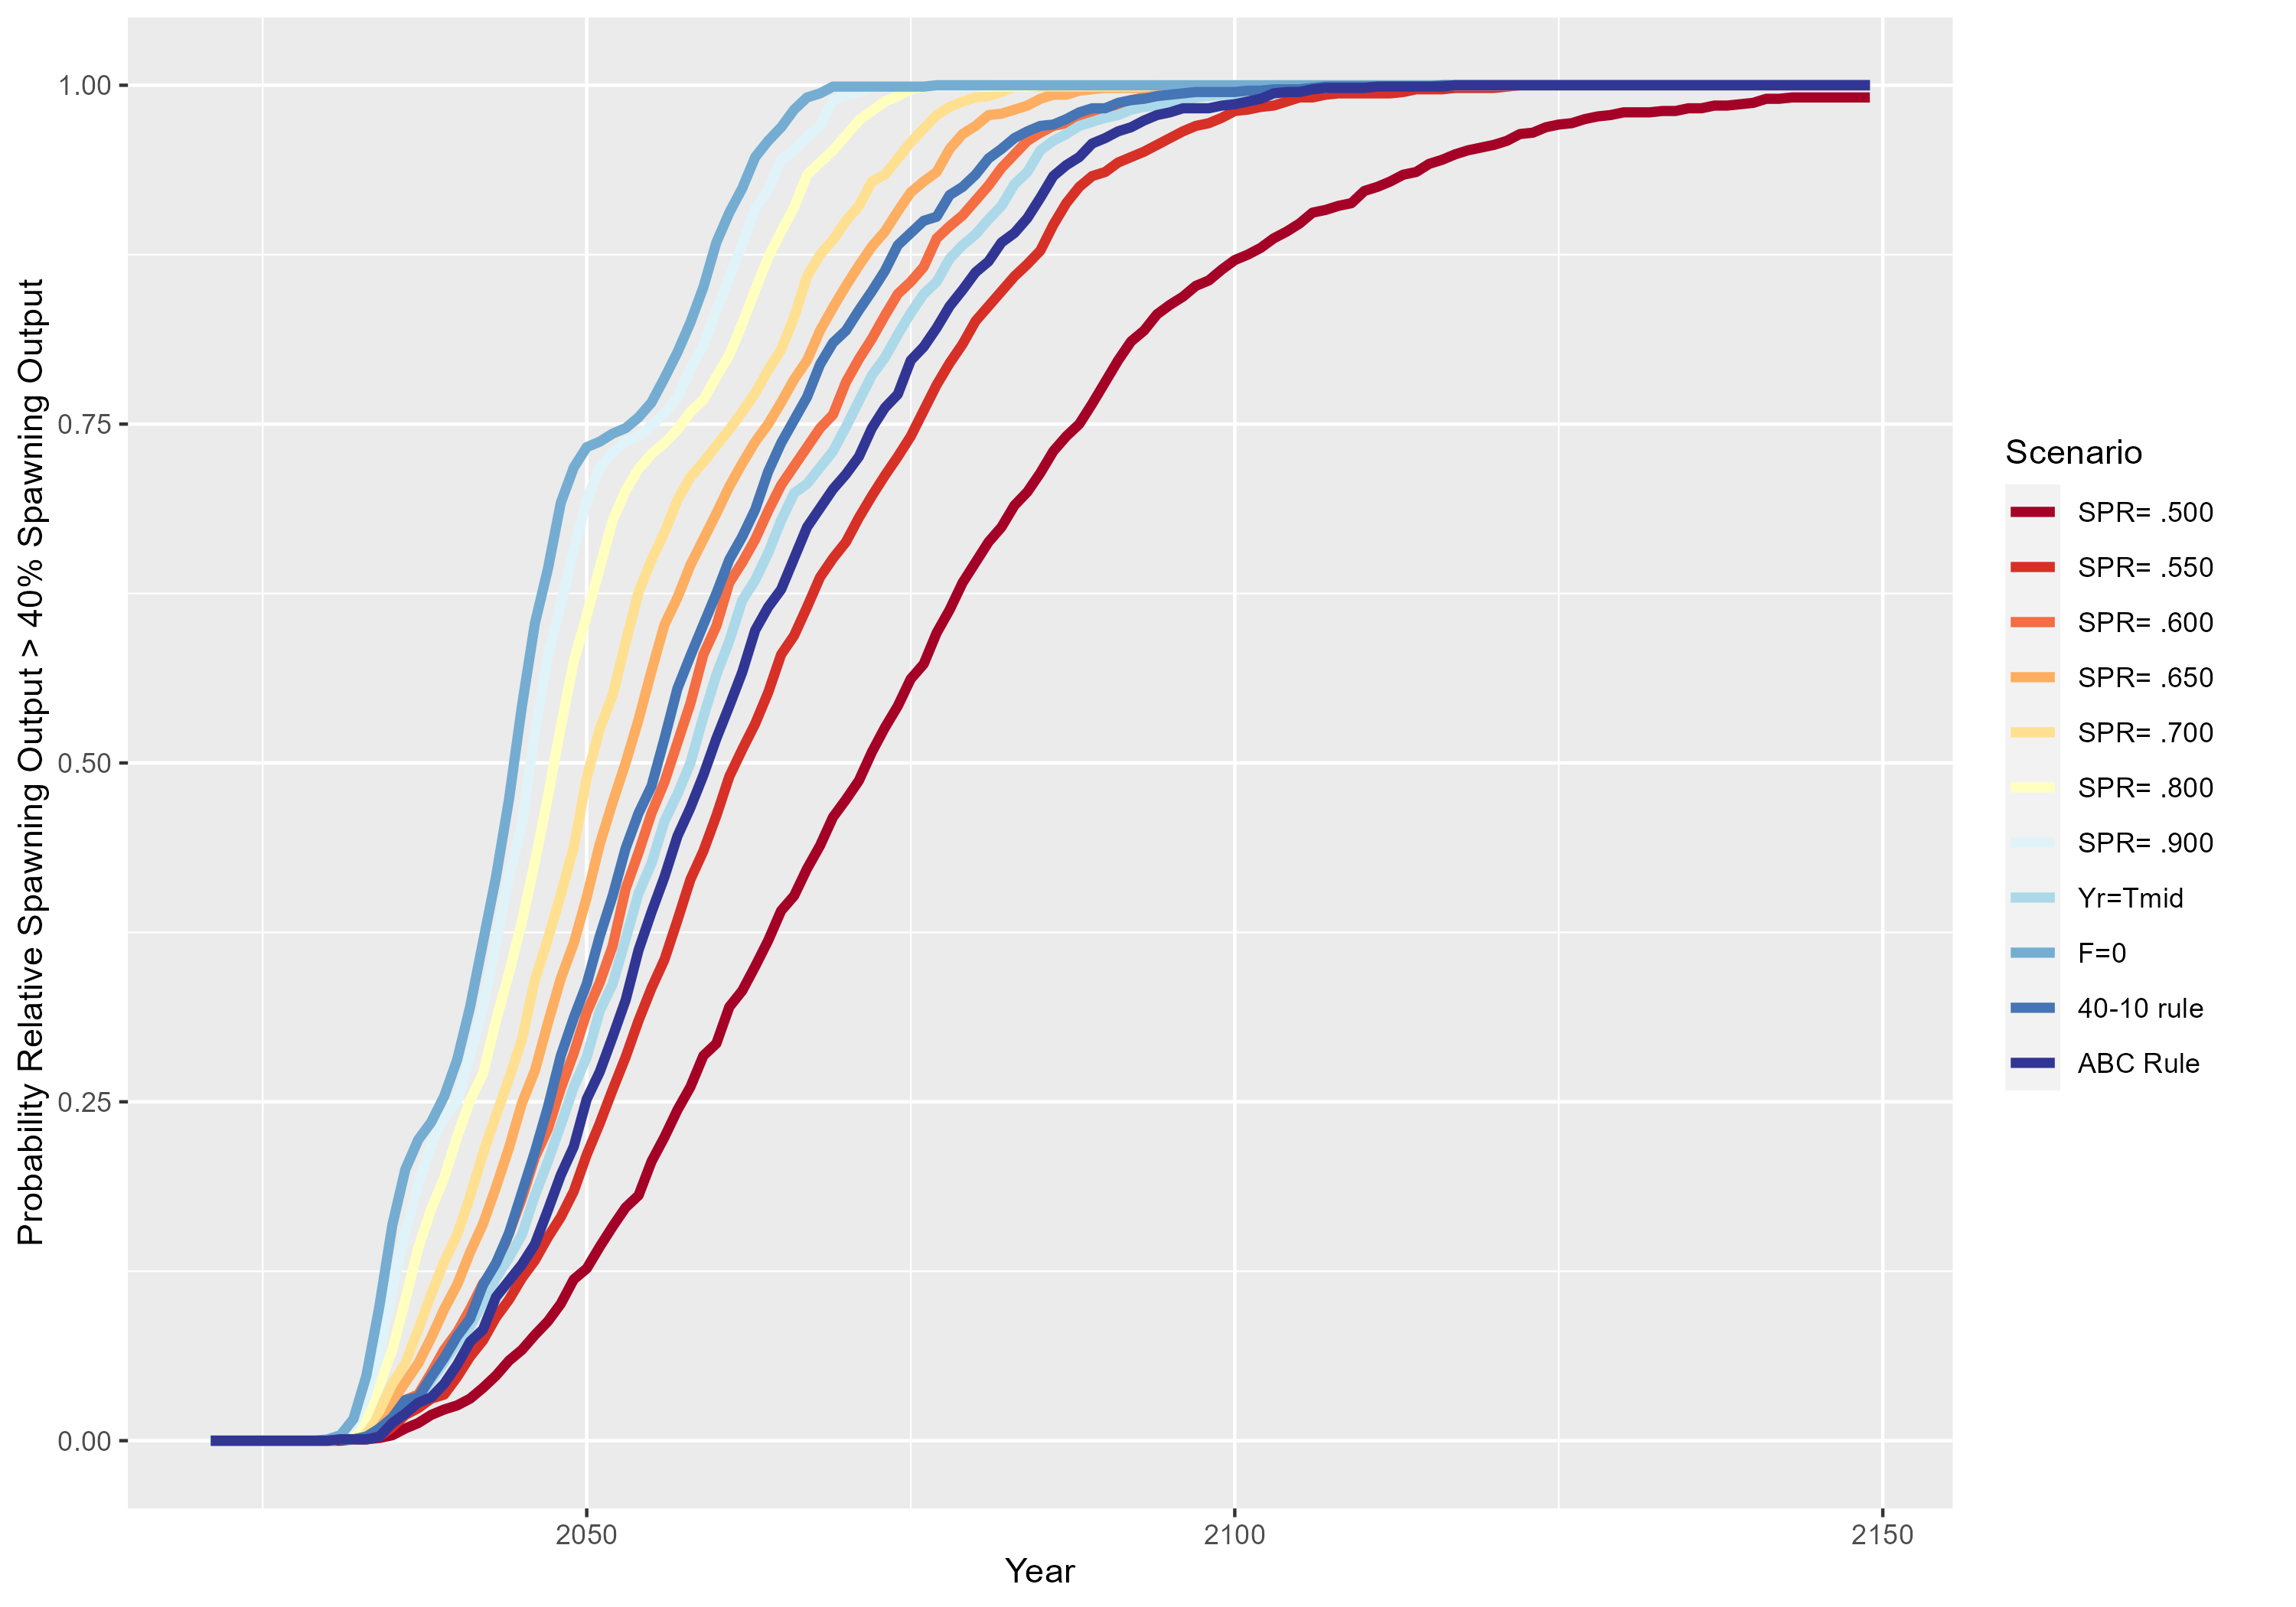
\includegraphics[width=1\textwidth,height=1\textheight]{C:/Users/Brian.Langseth/Desktop/ca/rebuilder/write_up_postNov/figures/rebuilding_probability_forREPORT.png}
\caption{Probability of rebuilding by year for the alternative rebuilding strategies, including ramp strategies.\label{fig:prob-fig}}
\end{figure}

\tagmcend\tagstructend

\tagstructbegin{tag=Figure,alttext={Line plot of catches by year after 2022 showing 13 lines that represent each rebuilding strategy.}}\tagmcbegin{tag=Figure}

\begin{figure}
\centering
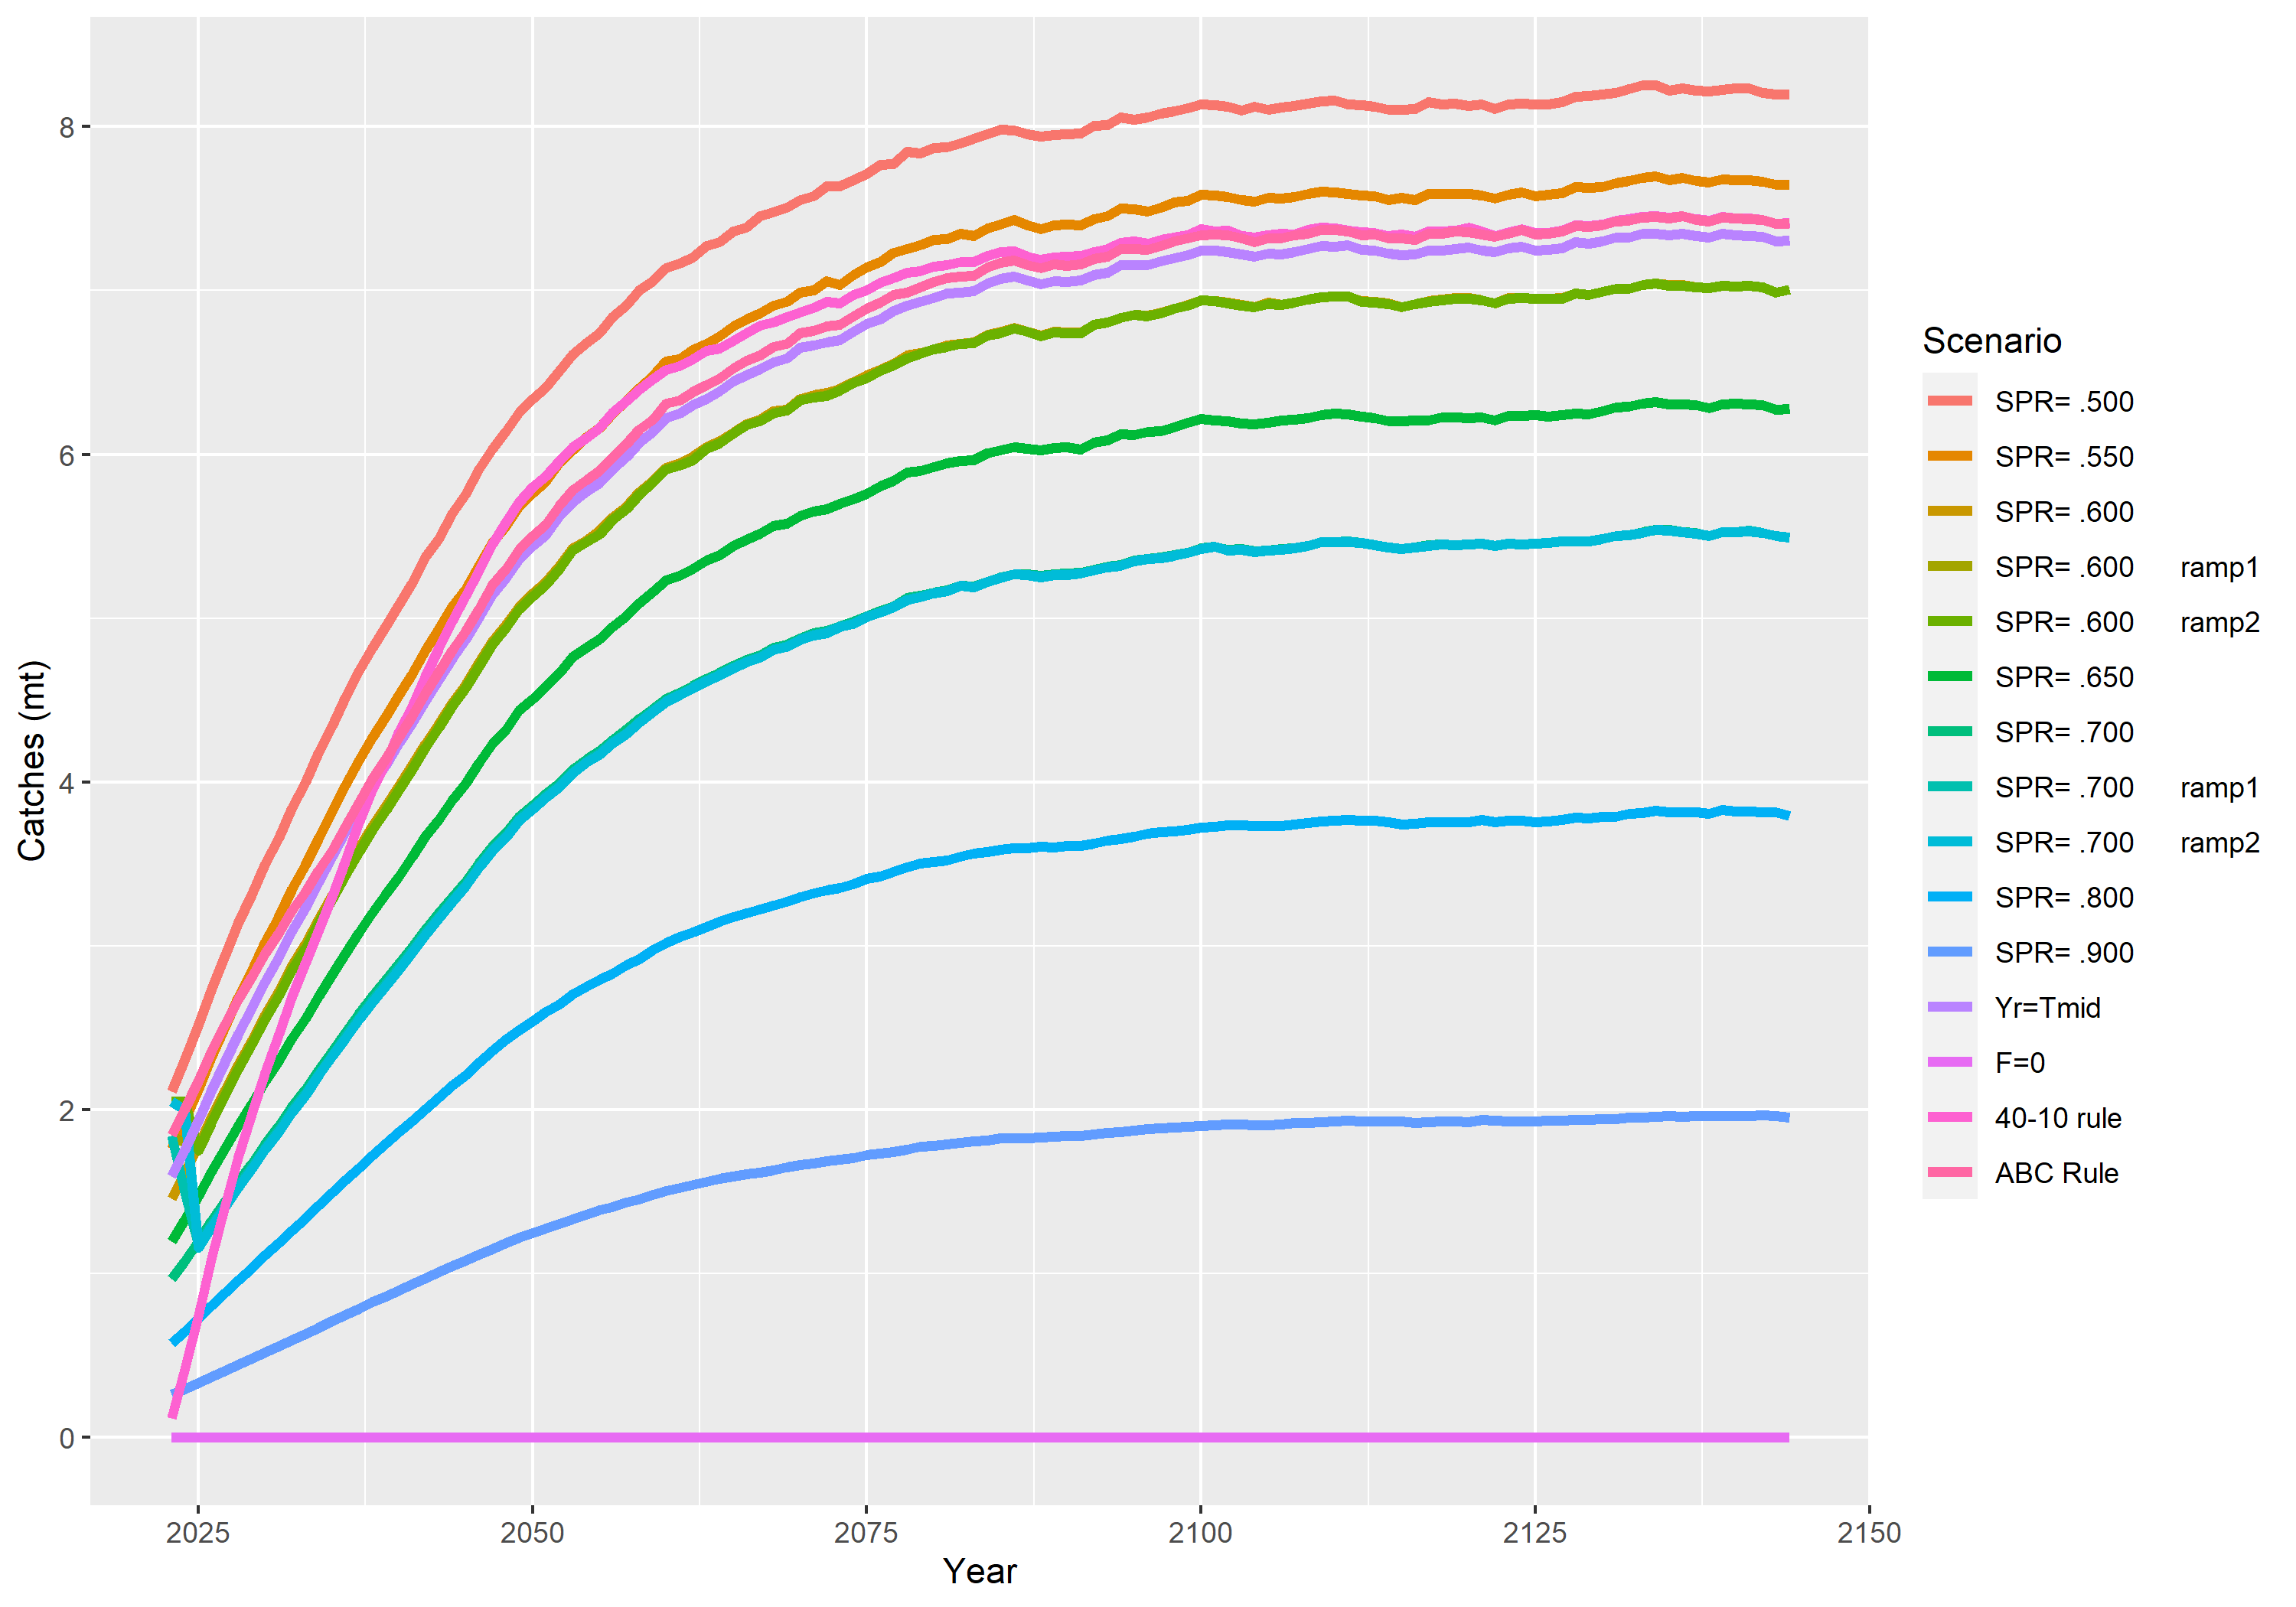
\includegraphics[width=1\textwidth,height=1\textheight]{C:/Users/Brian.Langseth/Desktop/ca/rebuilder/write_up_postNov/figures/rebuilding_acl_forREPORT.png}
\caption{Catches (mt) by year, starting in 2023, for the alternative rebuilding strategies, including ramp strategies.\label{fig:acl-fig}}
\end{figure}

\tagmcend\tagstructend

\tagstructbegin{tag=Figure,alttext={Line plot of relative spawning output by year after 2022 showing 13 lines that represent each rebuilding strategy.}}\tagmcbegin{tag=Figure}

\begin{figure}
\centering
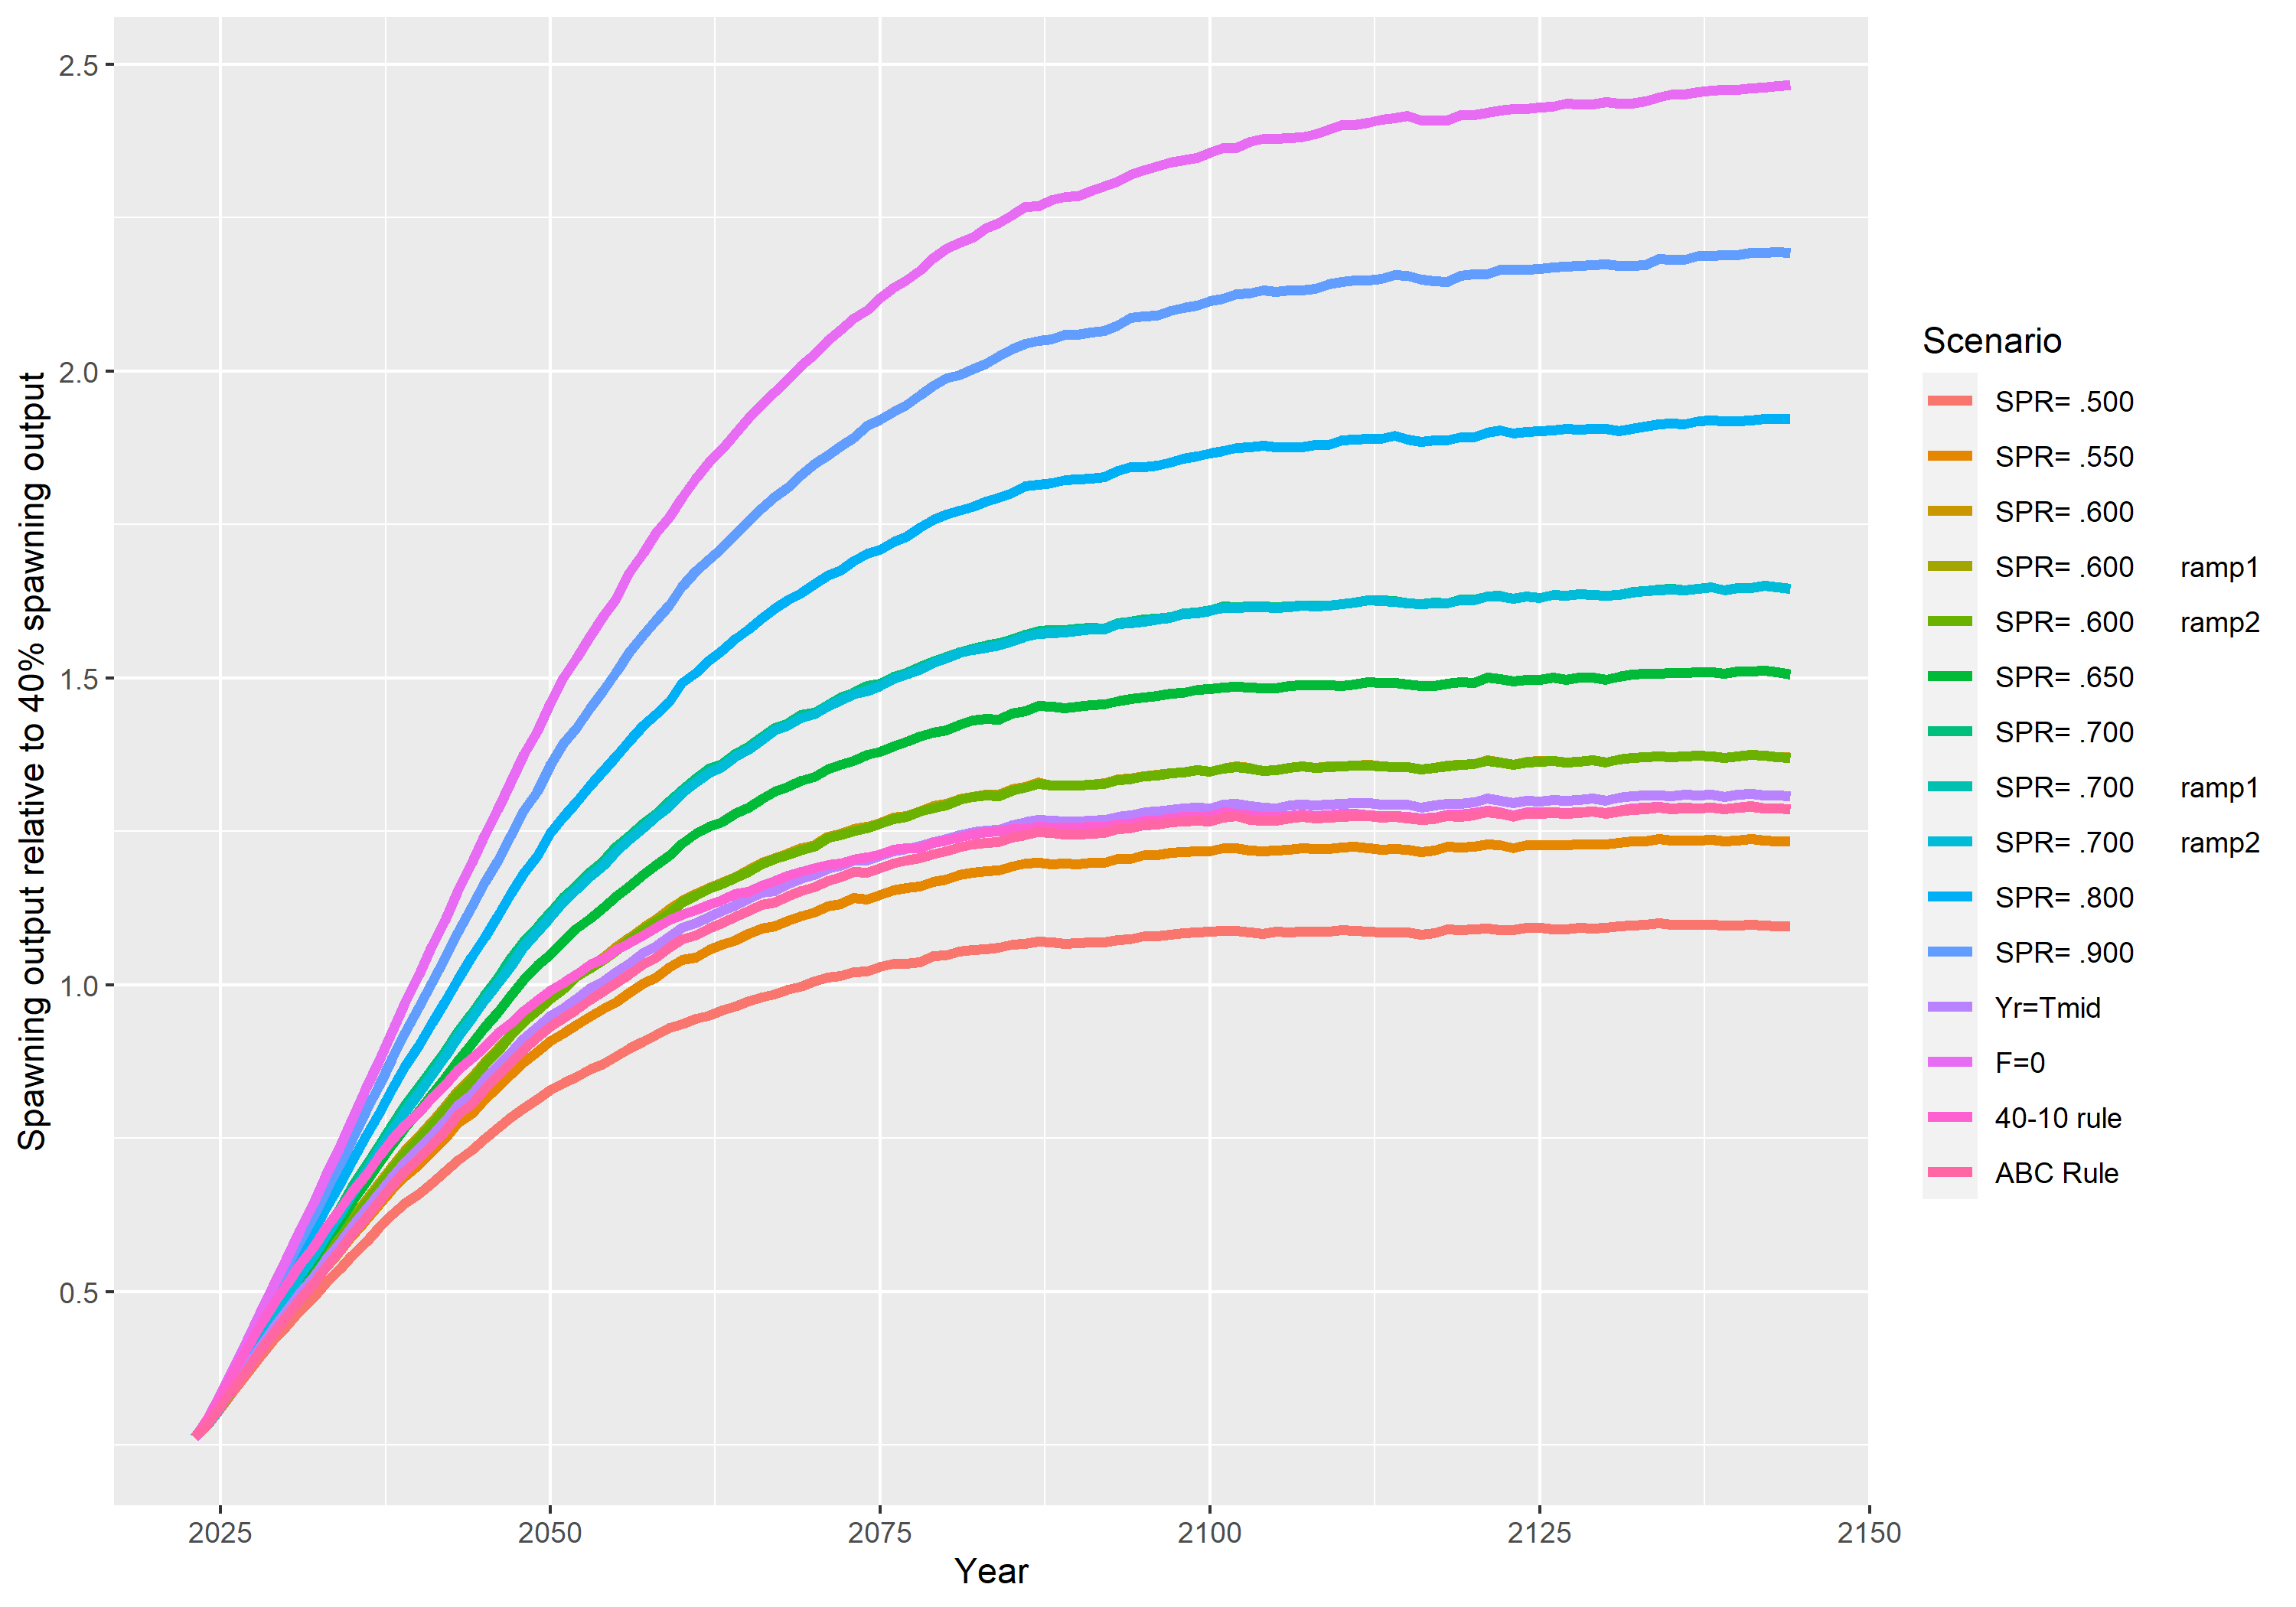
\includegraphics[width=1\textwidth,height=1\textheight]{C:/Users/Brian.Langseth/Desktop/ca/rebuilder/write_up_postNov/figures/rebuilding_relative_sb_forREPORT.png}
\caption{Spawning output relative to the management target of 40 percent of unfished spawning output by year, starting in 2023, for the alternative rebuilding strategies, including ramp strategies.\label{fig:rel-ssb-fig}}
\end{figure}

\tagmcend\tagstructend

\tagstructbegin{tag=Figure,alttext={Line plot of spawning output by year after 2022 showing 13 lines that represent each rebuilding strategy.}}\tagmcbegin{tag=Figure}

\begin{figure}
\centering
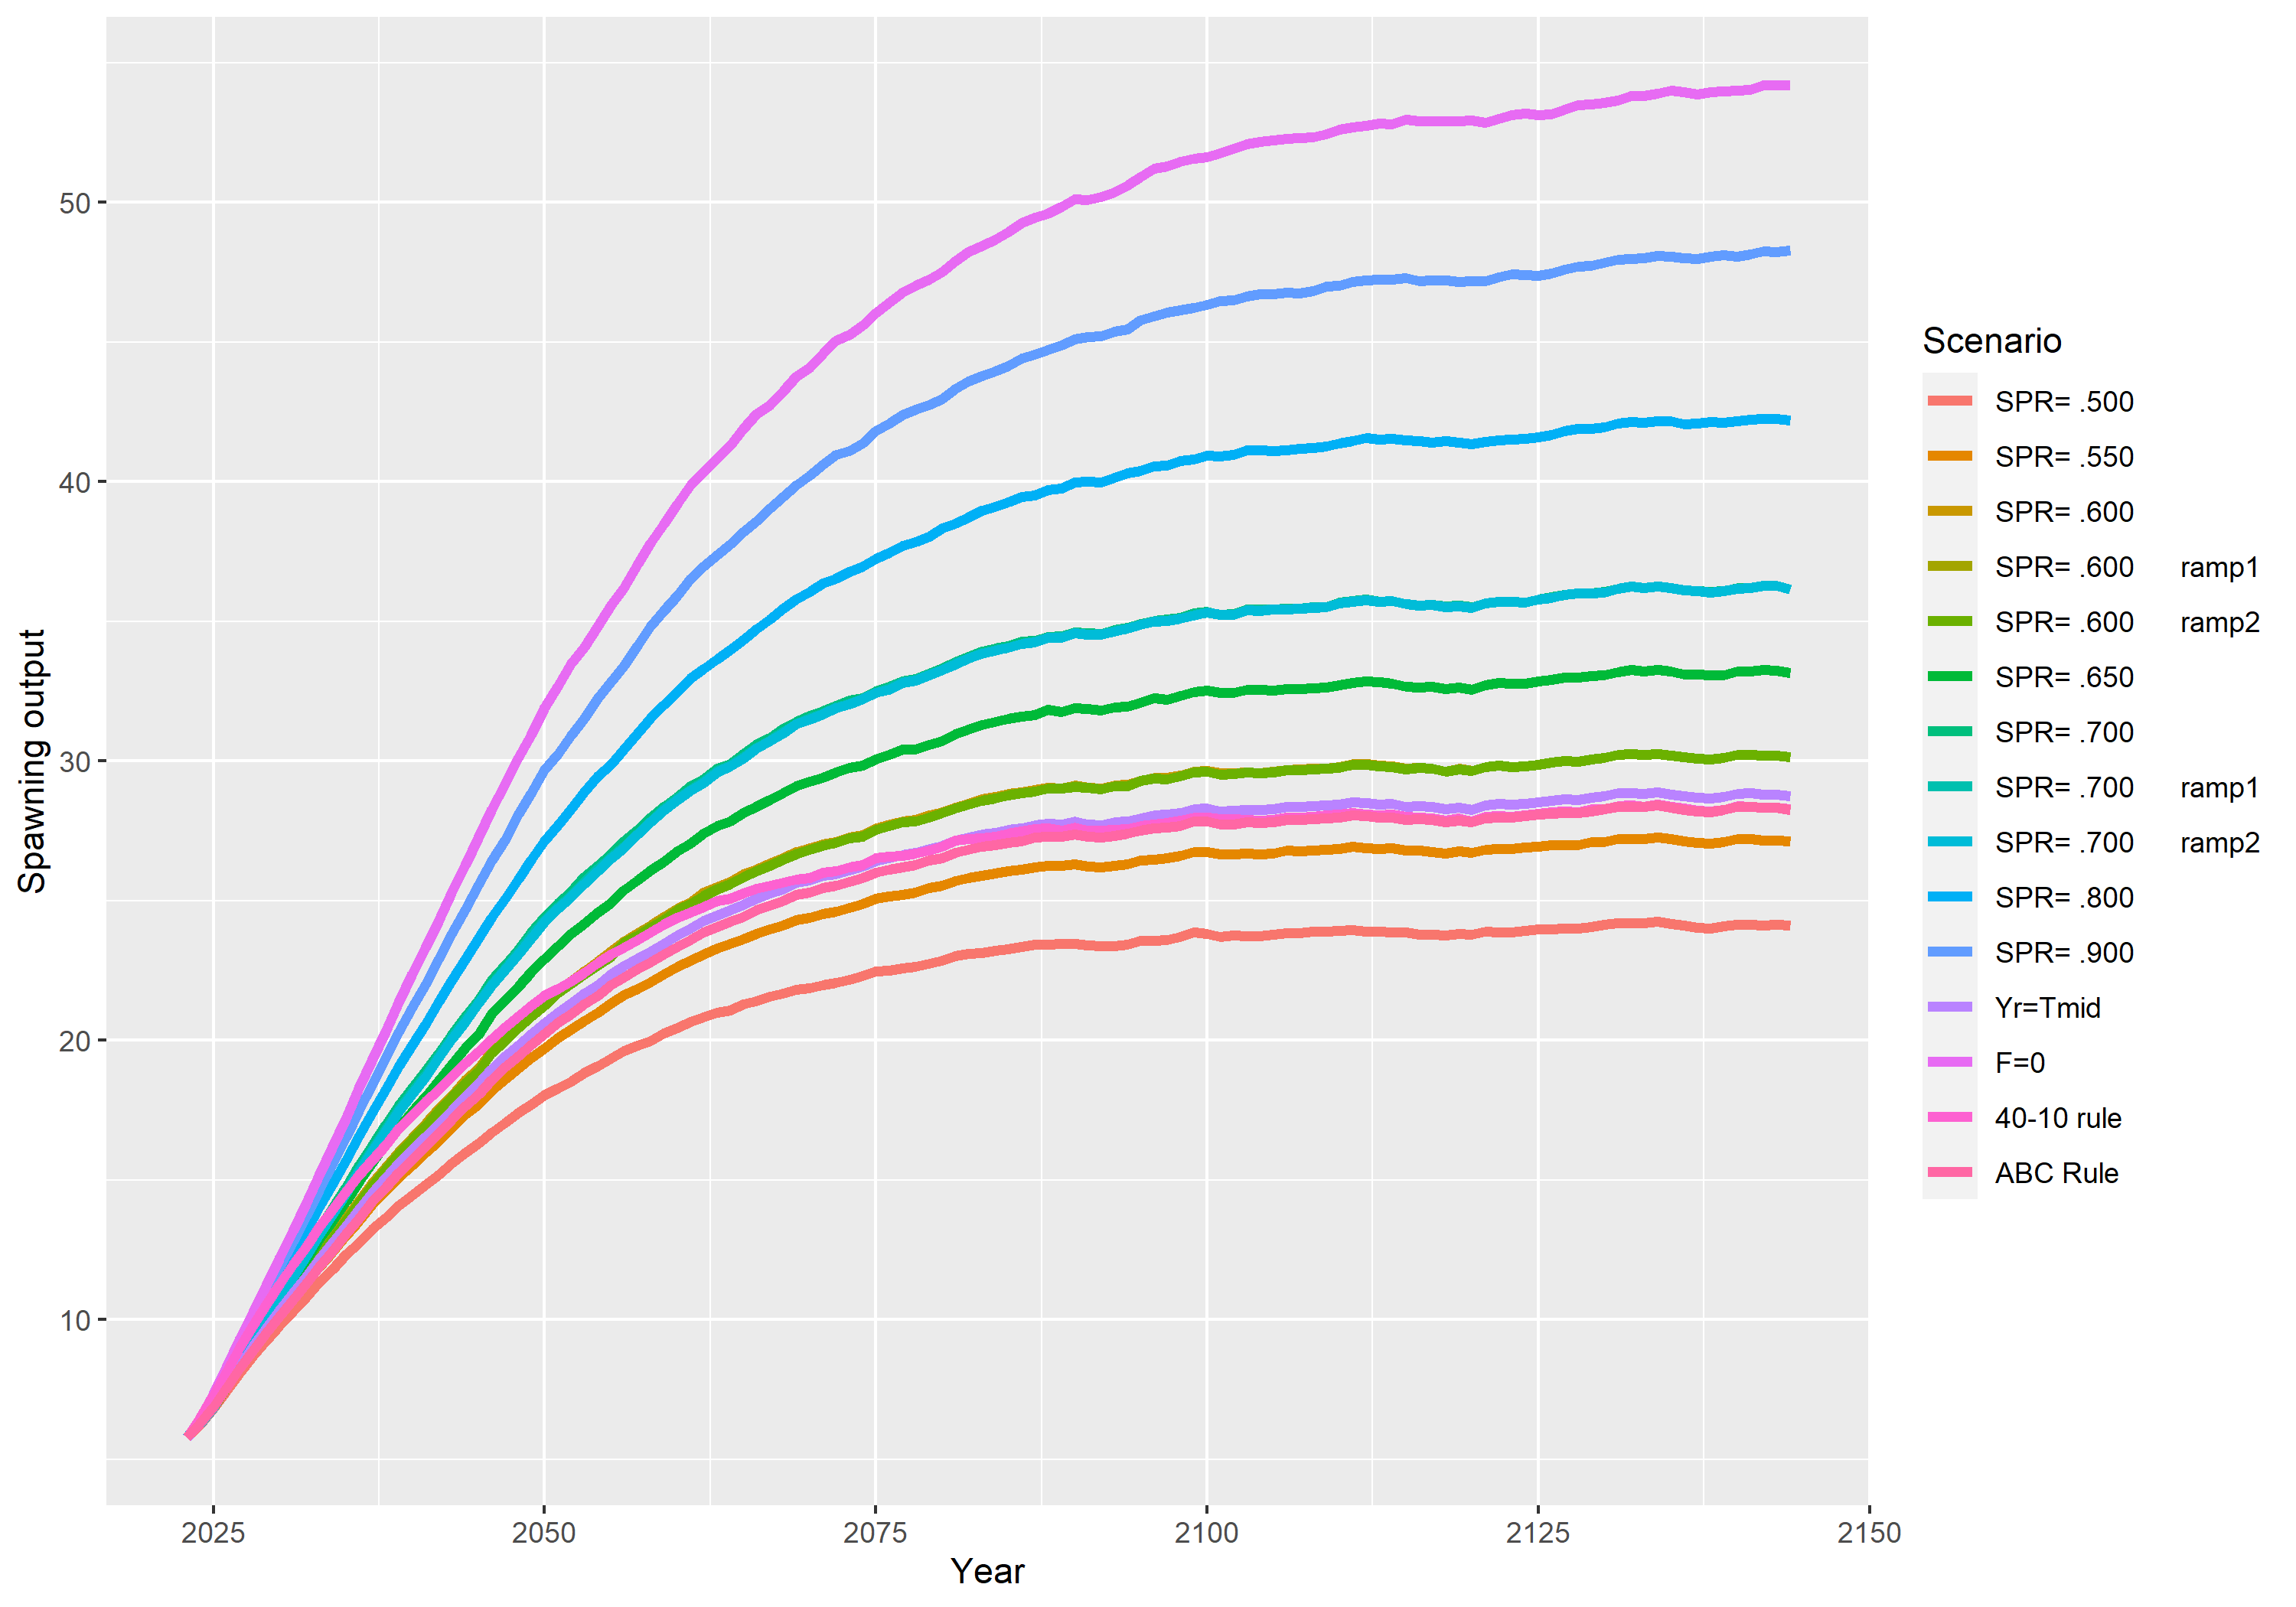
\includegraphics[width=1\textwidth,height=1\textheight]{C:/Users/Brian.Langseth/Desktop/ca/rebuilder/write_up_postNov/figures/rebuilding_ssb_forREPORT.png}
\caption{Spawning output by year, starting in 2023, for the alternative rebuilding strategies, including ramp strategies.\label{fig:ssb-fig}}
\end{figure}

\tagmcend\tagstructend

\clearpage

\clearpage

\tagstructbegin{tag=H1}\tagmcbegin{tag=H1}

\hypertarget{appendix}{%
\section{Appendix}\label{appendix}}

\leavevmode\tagmcend\tagstructend

\tagstructbegin{tag=H2}\tagmcbegin{tag=H2}

\hypertarget{append_a}{%
\subsection{Appendix A: Rebuilder data file.}\label{append_a}}

\leavevmode\tagmcend\tagstructend

\tagstructbegin{tag=P}\tagmcbegin{tag=P}

The rebuild.dat file used for the base rebuilding analysis has been provided as a separate file.

\leavevmode\tagmcend\tagstructend\par

\clearpage
\end{document}
